\chapter{Introducción}
	\label{cap:int}
	Un carpintero desea medir la distancia de una barra de madera que luego será, tal vez, la altura de las patas de una futura mesa. Para ello, utiliza una cinta métrica, compuesta de una cinta metálica que posee una escala graduada. Sabe entonces que la barra mide la distancia que coincide con la distancia de la cinta graduada.\\

Un panadero desea medir cuanto pesa la harina que debe para poder amasar. Entonces, la coloca en una balanza y observa cuanto marca su indicador. Así conoce que la masa de la harina es equivalente a la fracción de medida que indica la balanza.\\

Un atleta desea conocer cuanto demora en correr un trayecto que posee \SI{1}{\kilo\metro}. Por esto, registra el valor que indica su reloj al principio del recorrido y cuando alcanza el final observa nuevamente el artefacto. Luego de esto, calcula la diferencia entre el valor final y el inicial, conociendo cuanto tiempo le tomó realizar su travesía.\\

En los tres casos anteriores, tanto el carpintero, como el panadero y el atleta desconocen algo y necesitan cambiar su estado con respecto a esa incertidumbre. Por ello recurren a diferentes objetos, a fin de obtener conocimiento a partir de ellos. Sin embargo, estos objetos, por si mismos, no otorgan información, sino más bien otorgan un dato, que comparado y contrastado con otros datos, se traducen en conocimiento.\\

La información es el resultado de ordenar y procesar un conjunto de datos, de forma tal que permitan cambiar el estado de conocimiento sobre un asunto determinado. En el caso del carpintero, compara el tamaño de las patas de la mesa con una cinta metlálica, que a su vez, posee registrada su distancia en función de algún patrón de metrología, establecido por convención. Esto quiere decir que el dato 1, la longitud del patron, junto al dato 2, escala graduada de la cinta, más el dato 3, la longitud de la cinta métrica, permiten al carpintero cambiar su estado de desconocido a conocido, con respecto a la longitud del trozo de madera, a través de la información proporcionada por el conjunto de datos.\\

Se puede realizar el mismo análisis con respecto a la balanza del panadero, considerando un peso patrón, un desplazamiento y una escala graduada o una señal eléctrica emitida por una celda de carga deformada un porcentaje de su capacidad, registrada previamente por su fabricante conforme a pesos patrones, y un circuito adaptador que transforma esa señal electrica en un valor numérico mostrado en un indicador.\\

El atleta compara las posiciones y los desplazamientos de las agujas de su reloj, previamente calibrado para que dé una vuelta por cada minuto en una aguja, otra aguja que dé una vuelta por hora y la tercera una vez cada 12 horas. Además, es probable que él haya ajustado la hora que indica el reloj para que otorgue un horario idéntico al de referencia, establecido por convención.\\

En todos los casos, se posee una gran cantidad de datos que, ordenados, procesados y comparados otorgan al usuario un valor útil, ya sea una longitud, una masa, un tiempo o cualquiera sea la variable física que se desee conocer.\\

La ciencia es un conjunto de técnicas y procedimientos que, a través del método científico, busca adquirir, descubrir y/o desarrollar nuevo conocimiento. Se desprende entonces, que la ciencia produce, de forma fundamental, información que luego es transformada en conocimiento. Cuando hablamos de ciencia, hablamos de una gran gama de objetos de estudio, sujeto a través del cuál se clasifican, en la mayoría de los casos, las ciencias: las Ciencias Sociales estudian las relaciones humanas, las Ciencias Naturales estudian objetos que se encuentran en la naturaleza, las Ciencias de la Tierra se enfocan en una rama más particular de la naturaleza, como lo son los minerales, la superficie terrestre, etc; y siguiendo así se puede encontrar un sinnuméro se ciencias. Sin embargo, toda ciencia necesita, para su correcta producción científica, adquirir una gran cantidad de datos que luego será nordenados, procesados y transformados en información y conocimiento.\\

La incorporación de una herramienta especialmente diseñada para el procesamiento de datos, como lo es la computadora, permite manejar un numero cada vez creciente de información.
Es por eso que se encuentra en desarrollo un gran número de sensores y dispositivos que permitan obtener cada vez más datos.\\

En este sentido, una de los desarrollo que se encuentran en boga es el sensores que adquieran imágenes. Como ejemplos podemos encontrar, entre muchos otros, el desarrollo de sensores de radiación[1], ultrasonografía[2], telescopía de objetos cercanos[3], imagenes de distancia[4].





[1][https://ieeexplore.ieee.org/abstract/document/8214376]
[2][http://www.idr.iitkgp.ac.in/jspui/bitstream/123456789/9068/1/NB15975_Abstract.pdf]
[3][https://ieeexplore.ieee.org/abstract/document/8396725]
[4][https://www.sciencedirect.com/science/article/pii/S0030402617316029]




El mundo actual, en el que vivimos inmersos, demanda y consume volumenes cada vez más grandes de información. Con solo hacer una rapida miradad en diarios, incluso no especilizados, se observa la importancia que poseen las ciencias y disciplinas que manejas la informacion, aquellas areas agrupadas dentro del conjunto Técnico de la Información y la Comunicación, o más ocnocido por sus siglas, TIC's.

Internet de las cosas , Big Data, Inteligencia Artificial, Redes Neuronales, Robótica, Domótica, entre otras, son areas en las que los datos y la información es abultada y su correcto manejo es sumamente complejo e importante. Además, ninguna de las actividades científicas, puede escapar de esta gran demanda mundial de información.

La información es un conjunto de datos ordenados y procesados de forma tal que permita al que lo lea que eleve su nivel de conocimiento sobre un determinado tema. Es decir que, para que exista información, en primer lugar tenemos que tener datos, de forma tal que podamos luego procesarlos y obtener realmente información de llos.

Como ejemplo de esto, podemos citar simplemente el acto de medir la presión dentro de un tubo de gas. Sería normal pensar en que, teniendo este objetivo en mente, simplemente coloquemos un manómetro en la salida del tubo. El manómetro es un artefacto que posee una varilla 





El mundo, durante la era de la información, nos exige producir y consumir cada vez más y más información. En cada aspecto social dela vida de la persona se pueden encontrar ejemplos claros de esto.\\

Bajo un punto de vista social nos vemos bombardeados por información. Los 'influencers' que se mueven a traves de Facebook, Twiter, Instagram, Snapchat, Linkedin, Youtube, etc, necesitan para estar a la moda, producir constantemente material y que ese material sea consumido por alguien que este demandando esa información.

En el area de econimía y finanzas existen cada vez más robots que extraen información de las diferentes bolsas, periodicos, bancos, industrias y donde se ocurra que pueda haber información útil, para tomar mejores decisiones que, por supuesto, también ejecutan los robots.

En el comercio, desde las tiendas de supermercado hasta las tiendas digitales que trabajan solo a través de internet están constantemente recabando datos y procesandolos a din de diseñar estrategias que permitan ofrecer productos que se adapten mejor a lo que busca el cliente y de esa forma lograr vender mayores volumenes.

La industria cuenta cada vez más con multiplicidad de posibilidades basadas en sensores que adquieren grandes cantidades de datos que son almacenadas y procesadas, muchas vecen 'en línea' o 'al instante', de forma tal de encontrar mejores procesos o ejecutar nuevas tareas, como por ejemplo la industria automotriz, enfocada cada vez más en autos que puedan manipular todo el entorno y ser totalmente autónomos de un conductor.
La industria espacial y satelital dotan a sus equipos de mayores sensores y mayores flujos de datos. La industria médica brinda cada vez más posibilidades de diagnóstico a traves de nuevas técnicas y formas de adquisición de imágenes.

A todo esto, la ciencia y el desarrollo de nuevas aplicaciones y equipos, no son indiferente. Cada vez se encuentran más innovaciones y desarrollos de nuevos sensores que adquieren flujos de información crecientes. La toma de imagenes se ha vuelto una herramienta clave para la investigación en diversas areas, tales como la biología, la ciencia de materiales, las ciencias nucleares, las ciencias de la tierra, etc.

Las redes sociales son un ejemplo de esto, pero esto se observa en la industria, la economía, las finanzas e incluso hasta en la casa.



[1] file:///home/lechuzin/Facultad/Trabajo%20Final/lechuzing/docs/bibliografia/The-Rise-of-the-Network-Society-With-a-New-Preface-Volume-I-The-Information-Age-Economy-Society-and-Culture-Information-Age-Series-.pdf
	\section{Motivación}
		\label{int:mot}
		Un carpintero desea medir la distancia de una barra de madera que luego será, tal vez, la altura de las patas de una futura mesa. Para ello, utiliza una cinta métrica, compuesta de una cinta metálica que posee una escala graduada. Sabe entonces que la barra mide la distancia que coincide con la distancia de la cinta graduada.\\

Un panadero desea medir cuanto pesa la harina que debe para poder amasar. Entonces, la coloca en una balanza y observa cuanto marca su indicador. Así conoce que la masa de la harina es equivalente a la fracción de medida que indica la balanza.\\

Un atleta desea conocer cuanto demora en correr un trayecto que posee \SI{1.00}{\kilo\meter}. Por esto, registra el valor que indica su reloj al principio del recorrido y cuando alcanza el final observa nuevamente el artefacto. Luego de esto, calcula la diferencia entre el valor final y el inicial, conociendo cuanto tiempo le tomó realizar su travesía.\\

En los tres casos anteriores, tanto el carpintero, como el panadero y el atleta desconocen algo y necesitan cambiar su estado con respecto a esa incertidumbre. Por ello recurren a diferentes objetos, a fin de obtener conocimiento a partir de ellos. Sin embargo, estos objetos, por si mismos, no otorgan información, sino más bien otorgan un dato, que comparado y contrastado con otros datos, se traducen en conocimiento.\\

La información es el resultado de recopilar, ordenar y procesar un conjunto de datos, de forma tal que permitan adquirir mayor conocimiento sobre un asunto determinado y otorguen un significado mayor que cada uno de los datos por separado. En el caso del carpintero, compara el tamaño de las patas de la mesa con una cinta metlálica, que a su vez, posee registrada su distancia en función de algún patrón de metrología, establecido por convención. Esto quiere decir que el dato 1, la longitud del patron, junto al dato 2, escala graduada de la cinta, más el dato 3, la longitud de la cinta métrica, permiten al carpintero cambiar su estado de desconocido a conocido, con respecto a la longitud del trozo de madera, a través de la información proporcionada por el conjunto de datos.\\

Se puede realizar el mismo análisis con respecto a la balanza del panadero, considerando un peso patrón, un desplazamiento y una escala graduada o una señal eléctrica emitida por una celda de carga deformada un porcentaje de su capacidad, registrada previamente por su fabricante conforme a pesos patrones, y un circuito adaptador que transforma esa señal electrica en un valor numérico mostrado en un indicador.\\

El atleta compara las posiciones y los desplazamientos de las agujas de su reloj, previamente calibrado para que dé una vuelta por cada minuto en una aguja, otra aguja que dé una vuelta por hora y la tercera una vez cada 12 horas. Además, es probable que él haya ajustado la hora que indica el reloj para que otorgue un horario idéntico al de referencia, establecido por convención.\\

En todos los casos, se recopila una gran cantidad de datos que, ordenados, procesados y comparados otorgan al usuario una utilidad mayor que la del dato en sí, ya sea una longitud, una masa, un tiempo o cualquiera sea la variable física que se desee conocer.\\

La Ciencia es un conjunto de técnicas y procedimientos que, a través de un método científico, busca adquirir, descubrir y/o desarrollar nuevo conocimiento. Se desprende entonces, que la ciencia produce, de forma fundamental, datos, que luego de un procesado se transforman en información. A su vez, el estudio detallado de esta información genera conocimiento.\\

Cuando se nombra la palabra ciencia, se hace referencia a un conjunto conformado por diferentes objetos de estudio. El objeto de estudio es el sujeto a través del cuál se da la principal clasificación de las diferente ramas de la Ciencia: las Ciencias Sociales estudian las relaciones humanas y las Ciencias Naturales dedican sus esfuerzos a objetos que se encuentran en la naturaleza. Dentro del último grupo encontramos las Ciencias de la Tierra se enfocan en una rama más particular de la naturaleza, como lo es el estudio de la superficie terrestre; y siguiendo así se puede encontrar muchas más clasificaciones de ciencias, incluso como ramas englobadas por las anteriormente nombradas.\\

Sin embargo, la producción científica necesita adquirir una gran cantidad de datos que luego serán ordenados, procesados, analizados y transformados en información y conocimiento. En este sentido, la incorporación de una herramienta especialmente diseñada para el procesamiento de datos, como lo es la computadora, permite manejar un numero creciente de información. Es por eso que se encuentra en desarrollo un gran número de sensores y dispositivos que permitan obtener flujos crecientes de datos.\\

Uno de los desarrollo que se encuentra actualmente en boga es el de sensores y sistemas que adquieran imágenes de diferentes tipos. La captura de imágenes requiere de sistemas digitales de alta velocidad que tengan la capacidad de acarrear los datos desde el lugar físico en donde se obtienen los datos, es decir, en el transductor mismo, hasta el circuito o el sistema destinado al proceso de los mismos.\\

Para este tipo de aplicaciones, se torna de interés la utilización de un tipo particular de dispositivos electrónicos denominados FPGA ({\it Field-Programmable Gate Array}, o en español, Arreglo de Compuertas Programables en Campo), circuitos integrados programable para sintetizar circuitos digitales de alta velocidad. En otras palabras, este tipo de componentes permite implementar circuitos que ejecutan tareas complejas y resuelve problemas específicos.\\

Existen numerosos trabajos que utilizan FPGA para la producción de imágenes. Por ejemplo, el desarrollo de un sensor de radiación utilizando un sensor CMOS comercial. Para ello, los autores utilizaron un FPGA para configurar y transmitir imagenes a un grabador de video a través de puerto UART. Esto permitió adquirir una imagen a través de un disparador realizado con un pulsador\cite{Perez2017}.\\

Se denomina ultrasonografía a la técnica de adquirir imágenes basandose en rebotes de ultrasonido. Sus aplicaciones son múltiple, en las que se destaca el diagnóstico médico, ya que es una técnica no invasiva y sin riesgos de radiación ionizante sobre el paciente. Un trabajo reciente desarrolló un sistema de ecografía médica con bajo costo utilizando un FPGA\cite{biswas2018embedded}. El autor también presentó un algoritmo realizado y probado en PC. Luego se implementó e en una FPGA.\\

Existen sistemas de telescopía implementados con FPGA. Yanagisawa y otros desarrollaron un sistema con telescopios pequeños para explorar objetos de campo cercano con la finalidad de monitorear cuerpos celestes que puedan colisionar con el planeta\cite{Yanagisawa2018}. Los autores utilizan la velocidad de los circuitos implementados en FPGA para minimizar el tiempo de adquisición.

Existen sensores de imagenes de distancia desarrollados mediante FPGA\cite{Cui2018}.\\%BORRAR esta cita!!!

A diferencia de un microprocesador o un microcontrolador, también muy usados en la industria electrónica, en el cual una unidad logica algoritmica ejecuta un programa cargado secuencial, es decir, linea por línea, un FPGA puede ser programado de forma tal que cada proceso se ejecute en forma independiente y paralela, dotando al sistema de una mayor velocidad en el procesamiento.\\

De esta forma, un diseñador puede manipular un volumen mucho mayor de datos, que a los efectos de la adquisición y medición de imágenes, resulta más adecuado.\\

Pero como ya se mencionó con anterioridad, la obtención de datos por si misma no le otorga al científico la información, y por ende, el conocimiento nuevo que desea. Para ello, es probable que este gran flujo de datos requiera de un procesamiento y análisis más exhaustivo de los mismos.\\

Es por esto que la PC {\it Personal Computer} se ha transformado en la herramienta indispensable en cualquier ámbito, pero en especial en los entornos en donde se requiere el  manejo, cálculo, procesamiento y análisis de grandes cantidades de datos e información.\\

Se torna de suma utilidad, entonces, proveer una comunicación efectiva y robusta que permita mover grandes volúmenes de datos en poco tiempo, y de esta forma facilitar los tiempos de desarrollo, las pruebas y depuración de sistemas.\\

Desde la inclusión de la norma USB, en el año 1996 a la fecha, se ha convertido en el elemento que no falta en ningun equipo, al punto tal que ha desplazado a cualquier otro conector. Al punto tal es esto, que para requerir algún puerto adicional que no sea de esta norma, cualquier comprador debe especificar que así sea, mas no es necesario especificar que tiene USB como norma de conexión.\\

El presente trabajo pretende ofrecer una comunicación basada en la versión 2.0 de la norma USB entre una PC y un FPGA, y otorgue una herramienta adicional a científicos que desarrollen o utilicen sistemas basados en FPGA.\\
%
%Este trabajo, pretende elaborar una interfaz entre los dos extremos, es decir, entre la PFGA y la PC, de forma tal que permita a un desarrollador, investigador o usuario en general, obtener una comunicación confiable y con un ancho de banda que permita mover el flujo de datos que genera una sensor que adquiera imágenes.\\
%
%Es cierto que el protocolo puede ser totalmente implementado en una FPGA, sin embargo, esto requeriría un muy alto costo tanto económico como en recursos disponibles del chip programable para una tarea genérica que es mejor elaborar con un circuito integrado diseñado especialmente para tal fin. Es por esto que se utiliza como lazo de interfaz un chip comercial elaborado por Cypress Semiconductor.\\
%
%
%
%[1][https://ieeexplore.ieee.org/abstract/document/8214376]
%[2][http://www.idr.iitkgp.ac.in/jspui/bitstream/123456789/9068/1/NB15975_Abstract.pdf]
%[3][https://ieeexplore.ieee.org/abstract/document/8396725]




%El mundo actual, en el que vivimos inmersos, demanda y consume volumenes cada vez más grandes de información. Con solo hacer una rapida miradad en diarios, incluso no especilizados, se observa la importancia que poseen las ciencias y disciplinas que manejas la informacion, aquellas areas agrupadas dentro del conjunto Técnico de la Información y la Comunicación, o más ocnocido por sus siglas, TIC's.
%
%Internet de las cosas , Big Data, Inteligencia Artificial, Redes Neuronales, Robótica, Domótica, entre otras, son areas en las que los datos y la información es abultada y su correcto manejo es sumamente complejo e importante. Además, ninguna de las actividades científicas, puede escapar de esta gran demanda mundial de información.
%
%La información es un conjunto de datos ordenados y procesados de forma tal que permita al que lo lea que eleve su nivel de conocimiento sobre un determinado tema. Es decir que, para que exista información, en primer lugar tenemos que tener datos, de forma tal que podamos luego procesarlos y obtener realmente información de llos.
%
%Como ejemplo de esto, podemos citar simplemente el acto de medir la presión dentro de un tubo de gas. Sería normal pensar en que, teniendo este objetivo en mente, simplemente coloquemos un manómetro en la salida del tubo. El manómetro es un artefacto que posee una varilla 
%
%
%
%
%
%El mundo, durante la era de la información, nos exige producir y consumir cada vez más y más información. En cada aspecto social dela vida de la persona se pueden encontrar ejemplos claros de esto.\\
%
%Bajo un punto de vista social nos vemos bombardeados por información. Los 'influencers' que se mueven a traves de Facebook, Twiter, Instagram, Snapchat, Linkedin, Youtube, etc, necesitan para estar a la moda, producir constantemente material y que ese material sea consumido por alguien que este demandando esa información.
%
%En el area de econimía y finanzas existen cada vez más robots que extraen información de las diferentes bolsas, periodicos, bancos, industrias y donde se ocurra que pueda haber información útil, para tomar mejores decisiones que, por supuesto, también ejecutan los robots.
%
%En el comercio, desde las tiendas de supermercado hasta las tiendas digitales que trabajan solo a través de internet están constantemente recabando datos y procesandolos a din de diseñar estrategias que permitan ofrecer productos que se adapten mejor a lo que busca el cliente y de esa forma lograr vender mayores volumenes.
%
%La industria cuenta cada vez más con multiplicidad de posibilidades basadas en sensores que adquieren grandes cantidades de datos que son almacenadas y procesadas, muchas vecen 'en línea' o 'al instante', de forma tal de encontrar mejores procesos o ejecutar nuevas tareas, como por ejemplo la industria automotriz, enfocada cada vez más en autos que puedan manipular todo el entorno y ser totalmente autónomos de un conductor.
%La industria espacial y satelital dotan a sus equipos de mayores sensores y mayores flujos de datos. La industria médica brinda cada vez más posibilidades de diagnóstico a traves de nuevas técnicas y formas de adquisición de imágenes.
%
%A todo esto, la ciencia y el desarrollo de nuevas aplicaciones y equipos, no son indiferente. Cada vez se encuentran más innovaciones y desarrollos de nuevos sensores que adquieren flujos de información crecientes. La toma de imagenes se ha vuelto una herramienta clave para la investigación en diversas areas, tales como la biología, la ciencia de materiales, las ciencias nucleares, las ciencias de la tierra, etc.
%
%Las redes sociales son un ejemplo de esto, pero esto se observa en la industria, la economía, las finanzas e incluso hasta en la casa.
%
%
%
%[1] file:///home/lechuzin/Facultad/Trabajo%20Final/lechuzing/docs/bibliografia/The-Rise-of-the-Network-Society-With-a-New-Preface-Volume-I-The-Information-Age-Economy-Society-and-Culture-Information-Age-Series-.pdf
	\section{Protocolos disponibles para la transmisión de datos entre PC y FPGA}
		\label{int:pro}
		%PRESTAR ATENCION: pegado de archivo externo!!!

%ARCHIVO transmitir.tex modificado.

%Dada la motivación, se puede decir a priori que el objetivo del presente trabajo es la implementación de una efectiva comunicación entre una Computadora Personal (PC) y una FPGA. Sin embargo, este objetivo tan amplio se plasmará de forma más concreta y detallada en la Sección \ref{int:obj}.\\

%El estándar más exigente de la norma americana de la SCTE (Sociedad de Ingenieros de Comunicación por Cable) utilizada Televisión Digital, posee una tasa de \SI{38.8}{\mega\bit\per\second}~\cite{SocietyofCableTelecommuniocationsEngineers2006}. Por su parte, la serie de sensores para adquirir imágenes monocromáticas MT9M001, comercializado por ON Semiconductors posee 1280x1024 pixeles, con profundidad de 10 bits y puede operar hasta a 30 cuadros por segundo~\cite{MicronTechnology2004}. La tasa de transmisión necesaria es, por tanto, de \SI{310}{\mega\bit\per\second}.%\\
%¿Y cuál es el protocolo que mejor se ajusta a la necesidad de disponibilidad? 

Un requerimiento que normalmente se busca en periféricos informático es el de compatibilidad. No es conveniente utilizar puertos que requieran acceso a la placa madre de la \acrshort{pc}, como el caso de tarjetas de tipo PCI o PCI express, debido a que no todos los equipos los tienen accesible, como ser computadoras portátiles. Más aún, en algunos casos estos puertos pueden estar todos ocupados. Se opta, entonces, por alguno de los tres puertos de moda: Ethernet, dedicado principalmente a conexión de redes mediante cables; Wi-Fi, utilizado para el acceso a la red de forma inalámbrica; y \acrshort{usb}, dirigido a la comunicación de periféricos con la \acrshort{pc}.%\\
%Además, pensando en que la implementación sea compatible con equipos informáticos convencionales, es decir, se encuentren fácilmente en el mercado y no posean especificaciones que escapen al uso de oficina. Esto se cumple hoy en día con tres tipos de puertos: Ethernet, dedicado principalmente a conexión de redes mediante cables; Wi-Fi, utilizado para el accesos a la red de forma inalámbrica; y USB, dirigido a la comunicación de periféricos con la PC.\\

Al hablar de Ethernet o Wi-Fi, se hace referencia a dos formas diferentes de conectarse a una red de computadoras. En otras palabras, se habla de dos o más nodos, compuestos por \acrshort{pc}s o cualquier dispositivo electrónico con capacidad de realizar cálculo binario, que pueden intercambiar datos a través de una trama bastante compleja de componentes diferentes. Ambos protocolos hacen referencia solo a la conexión física de los dispositivos y el control de acceso de cada uno de ellos a la conexión. Queda a cargo de otros sistemas, con sus protocolos, que los datos enviados puedan ser correctamente recibidos por el usuario de la \acrshort{pc}. La gran diferencia entre ellos radica en el medio físico que utilizan: Wi-Fi emplea ondas electromagnéticas emitidas mediante radiofrecuencia, mientras que en Ethernet, estas ondas son transportadas a través de uno o más conductores, como ser cable coaxial, cables de par trenzado o fibra óptica.%\\

Ethernet, también conocido como IEEE 802.3, es una norma que define cómo se deben conectar nodos a través de conductores para conformar \acrlong{lan} (\acrshort{lan} o {\it Local Area Network}), es decir, redes pequeñas, como ser domésticas, de oficinas o de pequeñas empresas, de forma que puedan transmitir información a velocidades seleccionables entre \SI{1}{\mega\bit\slash\second} y \SI{400}{\giga\bit\slash\second}~\cite{Ethernet2018}. Utiliza una tecnología denominada \acrlong{csma} (\acrshort{csma} del inglés {\it Carrier Sense Multiple Access with Collision Detection}). En una red con \acrshort{csma}, cada dispositivo debe sensar en forma permanente la conexión a la red, es decir, no existe un dispositivo que dirija el uso del bus, sino que cada uno debe identificar el estado de la red. Los mensajes se envían modulados. Cuando una señal portadora es detectada, todos chequean la dirección del paquete de información que viaja y el mensaje es recibido solamente por el dispositivo que se corresponda con esa dirección. Siempre que exista una señal portadora en el bus, los dispositivos que deseen transmitir información deberán esperar a fin de evitar colisiones, o sea, que dos dispositivos envíen mensajes a la vez y estos se interfieran.%\\

%Ethernet, también conocido como IEEE 802.3, es una norma que define cómo se deben conectar nodos a través de conductores para conformar redes de área local (LAN o {\it Local Area Network}), es decir, redes pequeñas, como ser domésticas, de oficinas o de pequeñas empresas, de forma que puedan transmitir información a velocidades seleccionables entre \SI{1}{\mega\bit\slash\second} y \SI{400}{\giga\bit\slash\second} ~\cite{Ethernet2018}. Utiliza una tecnología denominada Acceso Múltiple Sensando la Portadora con Detección de Colisiones (CSMA/CD del inglés {\it Carrier Sense Multiple Access with Collision Detection}). Esta tecnología se caracteriza por la escucha activa de todos los dispositivos conectados a la red. Solo cuando la dirección del paquete de información que viaja corresponde al dispositivo, este realiza una función. A la hora de transmitir, corrobora que no exista una señal portadora y, si ésta está presente, espera para retransmitir.\\

Dependiendo de la frecuencia de la portadora y la tasa de transferencia a la que transporta el mensaje, la norma especifica el conector y la distancia máxima a la que debe conectarse una repetidora, es decir, un dispositivo que reciba, reconstruya y emita la señal recibida. Estos conectores pueden ser cable coaxial, fibra óptica o cable de par trenzado. Este último es el más usual en las \acrshort{pc} comerciales y se muestra, junto a su ficha característica en la Figura \ref{fig:utp}.%\\

\begin{figure}[b]
	\centering
	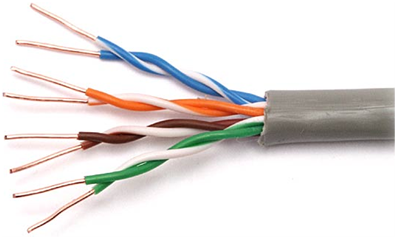
\includegraphics[width=0.4\textwidth]{partrenzado.png}
	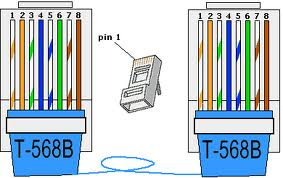
\includegraphics[width=0.4\textwidth]{utp.jpeg}
	\caption{Par Trenzado y un dibujo de su ficha de conexión.}
	\label{fig:utp}
\end{figure}

%La norma IEEE 802.3 también especifica cómo debe ser el formato de la información que se transmite, de forma tal que todas las velocidades, conectores y conductores sean compatibles entre si. Indica así que l
La información se estructura en paquetes para permitir la comunicación entre muchos nodos de la red. Un paquete, como se observa en la Figura \ref{fig:eth}, se compone de un preámbulo con \SI{7}{bytes} (B) que sirve para sincronizar los dispositivos en cada extremo de la conexión, \SI{1}{\byte} de inicio, \SI{12}{\byte} de direcciones, que corresponden 6 al nodo destinatario y 6 al emisor respectivamente, \SI{2}{\byte} que indican la longitud del mensaje, entre 46 y \SI{1500}{\byte} de datos y \SI{4}{\byte} para la verificación de la transmisión. Otra definición importante de la norma, son las características eléctricas de las señales, pero no se detallan en este trabajo porque varían en función de la velocidad del puerto.%\\


\begin{figure}[t]
	\centering
	\begin{adjustbox}{width=0.6\textwidth}
		\begin{tikzpicture}
		\begin{scope}[transform shape,node distance=.05,>=latex]
		\node[field](pa){PA};
		\node[field](init)[right=of pa]{IP};
		\node[field](dest)[right=of init]{DD};
		\node[field](emit)[right=of dest]{DE};
		\node[field](long)[right=of emit]{LM};
		\node[field](msj)[right=of long]{Mensaje};
		\node[field](crc)[right=of msj]{SCP};
		\end{scope}
		\begin{scope}[transform shape, node distance=.01]
		\node[](patx)[below=of pa]{7};
		\node[node distance=.2](bytes)[left=of patx] {\bf Bytes};
		\node[](inittx)[below=of init]{2};
		\node[](desttx)[below=of dest]{6};
		\node[](emittx)[below=of emit]{6};
		\node[](longtx)[below=of long]{2};
		\node[text width=50](patx)[below=of msj]{46 a 1500};
		\node[](msjtx)[below=of crc]{4};
		\node[node distance = 1](addtx)[below=of dest.east |- emit.west] {Direcciones};
		\draw[decoration={brace,mirror,raise=14pt},decorate](dest.south west) to (emit.south east);
		\end{scope}
		\begin{scope}[transform shape,node distance=.4,text width = 210]
		\node[below=of desttx](ref){
			{\bf Referencias}\\
			{\bf PA:}Pre{\'a}mbulo\\
			{\bf IP:} Inicio de Paquete\\
			{\bf DD:} Direcci{\'o}n de Destino\\
			{\bf DE:} Direcci{\'o} de Emisi{\'o}n\\
			{\bf LM:} Longitud del Mensaje\\
			{\bf SCP:} Secuencia de chequeo del paquete
		};
		\end{scope}
		\end{tikzpicture}
	\end{adjustbox}
	\caption{Estructura de un paquete Ethernet}
	\label{fig:eth}
\end{figure}

Por su parte Wi-Fi, perteneciente a la asociación de compañías denominada Wi-Fi Alliance, se rige por la norma que estableció esta última. Existe una norma equivalente, encuadrada en la especificación IEEE 802.11, referida a las \acrlong{wlan}, (\acrshort{wlan}, siglas del inglés {\it Wireless Local Area Network}). Wi-Fi se enfoca en las que se refieren a las comunicaciones de radiofrecuencia con portadora de \SI{2,4}{\giga\hertz}, que se incorporan en las revisiones b, g y n de la norma IEEE. IEEE 802.11 está pensado especialmente para dispositivos portátiles y móviles. La norma define a los dispositivos portátiles como aquellos que pueden ser trasladados con facilidad pero operan estáticos y los móviles se identifican por poder trabajar en movimiento~\cite{wifi2016}. La principal característica que posee este tipo de comunicación es la falta de conductores para la elaboración de la red, sin contar las conexiones entre los transceptores que emiten y reciben las señales de radiofrecuencias y los nodos, en donde la información es producida y/o consumida. En cuanto al formato del paquete de datos, el cual se muestra en la Figura \ref{fig:wifi}, es bastante similar al de Ethernet. En primer lugar, se envían \SI{2}{\byte} de control que indican el tipo de paquete a enviar. Luego siguen \SI{2}{\byte} que, dependiendo de la etapa de la comunicación puede indicar la duración del mensaje a transmitir o un identificador de una conexión establecida previamente. Siguen entre \si{6} y \SI{18}{\byte} de direcciones del enrutador que recibe los datos, el nodo emisor y el destinatario. Continúan, \SI{2}{\byte} de control de secuencia que se utilizan para fragmentar transmisiones largas. Continua un campo más para dirección que corresponde a la red emisora de \SI{6}{\byte}. Todos los campos de dirección pueden variar en función del tipo de mensaje que se envía. Los últimos dos campos de la trama corresponden a la información que se quiere comunicar (hasta \SI{2312}{\byte}) y un código de chequeo por redundancia cíclica de \SI{32}{\bit} (\SI{4}{\byte}).%\\

\begin{figure}[t]
	\centering
	\begin{adjustbox}{width=0.7\textwidth}
		\begin{tikzpicture}[]
		\begin{scope}[transform shape,node distance=.05,>=latex]
		\node[field](cp){CP};
		\node[field](dcid)[right=of cp]{Dur/CID};
		\node[field](routd)[right=of dcid]{DED};
		\node[field](dest)[right=of routd]{DD};
		\node[field](emit)[right=of dest]{DE};
		\node[field](cseq)[right=of emit]{CS};
		\node[field](route)[right=of cseq]{DEE};
		\node[field](msj)[right=of route]{Mensaje};
		\node[field](crc)[right=of msj]{SCP};
		\end{scope}
		\begin{scope}[transform shape, node distance=.01]
		\node[](cptx)[below=of cp]{2};
		\node[node distance=.2](bytes)[left=of cptx] {\bf Bytes};
		\node[](dcidtx)[below=of dcid]{2};
		\node[](routdtx)[below=of routd]{6};
		\node[](desttx)[below=of dest]{6};
		\node[](emittx)[below=of emit]{6};
		\node[](cseqtx)[below=of cseq]{2};
		\node[](routetx)[below=of route]{6};
		\node[text width=50](patx)[below=of msj]{variable};
		\node[](msjtx)[below=of crc]{4};
		\node[node distance = .5](addtx)[below=of dest] {Direcciones};
		\draw[decoration={brace,mirror,raise=14pt},decorate](routd.south west) to (emit.south east);
		\end{scope}
		\begin{scope}[transform shape,node distance=.4,text width = 320]
		\node[below=of desttx](ref){
			{\bf Referencias}\\
			{\bf CP:} Control de Paquete\\
			{\bf Dur/CID:} Duraci{\'o}n del paquete/Identificaci{\'o}n de conexi{\'o}n\\
			{\bf DED*:} Direcci{\'o}n de Enrutador de Destino\\
			{\bf DD*:} Direcci{\'o}n de Destino\\
			{\bf DE:} Direcci{\'o}n de Emisi{\'o}n\\
			{\bf CS*:} Control de Secuecia\\
			{\bf DEE*:} Direcci{\'o}n de Enrutador de Emisión\\
			{\bf SCP:} Secuencia de chequeo del paquete\\
			{\scriptsize *Pueden no estar dependiendo del tipo de mensaje}
		};
		\end{scope}
		\end{tikzpicture}
	\end{adjustbox}
	\caption{Estructura de un paquete Wi-Fi}
	\label{fig:wifi}
\end{figure}

Existen múltiples ventajas de utilizar radiofrecuencias para conectarse a la red, tales como la libertad de mover el punto de trabajo y la economía a la hora de armar redes con muchos nodos. Sin embargo, posee algunas desventajas notorias, propias del medio de propagación, que lo hacen no tan óptimo para los fines del presente trabajo. Las redes inalámbricas tienen la característica de que no son del todo confiables: poseen múltiples fuentes de interferencia, ya que varias tecnologías utilizan la misma frecuencia (Bluetooth, Zig-Bee, WUSB, microondas). A su vez, suelen presentar variaciones temporales y asimetrías en las propiedades de propagación, lo que puede provocar interrupciones en la comunicación.%\\

Ambos protocolos proporcionan una solución de conexión de redes de nivel físico y ejecutan tareas de \acrfull{mac} a fin de evitar colisión en los datos, es decir, que dos dispositivos transmitan en forma simultánea e interfieran la comunicación.
Sin embargo, para establecer una red, faltan componentes físicos y lógicos tales como el sistema de \acrfull{llc}, un sistema de direccionamiento, como el \acrfull{ip}, una capa de transporte de datos, como el \acrfull{tcp} y las capas de software que permiten acceder a los protocolo anteriormente mencionados.%\\

A pesar de lo anterior, es posible establecer comunicaciones punto a punto con ambos protocolos, simplificando mucho el sistema de transmisión de datos. Sin embargo estas soluciones presentan un inconveniente no menor: se le quita a la \acrshort{pc} un acceso a la red, que en la mayoría de los casos es el único. Esto no es deseable ya que la conectividad es un requisito fundamental en cualquier hogar u organización, ya sea empresarial, gubernamental, científica o de cualquier tipo.%\\

Por su parte el protocolo \acrshort{usb} (acrónimo de {\it Universal Serial Bus}), es una norma desarrollada por seis de las empresas más grandes de la industria informática, pensada y desarrollada para la conexión de teléfonos y periféricos a \acrshort{pc}s~\cite{USBspec}. En la versión original, \acrshort{usb} posee conectores cableados de 4 conductores y presenta una topología de bus, es decir todos los dispositivos se conectan a un mismo circuito conductor. La conexión es manejada por una \acrshort{pc} y solo transmite o recibe un dispositivo a la vez. Tal fue la penetración de \acrshort{usb} en el mercado, que se transformó en una norma de facto. Actualmente es incorporada casi por defecto en casi todas las computadoras disponibles en el mercado y es necesaria a la hora de comprar e instalar periféricos.%\\
%Si bien se puede implementar la comunicación vía Ethernet, cumpliendo con las especificaciones propuestas, es muy probable que el único puerto que posea la PC se encuentre conectado a la red y se necesitará una infraestructura mayor para lograr una efectiva comunicación. Por tanto, USB se observa como una solución óptima.\\

\acrshort{usb} presenta diferentes versiones de su norma, cada cual con una o más tasas de transmisión y señalización. La versión 1 posee dos revisiones, 1.0 fue lanzada al mercado en el año 1996 y 1.1 que se presentó en Agosto de 1998. La primera alcanza una tasa máxima de \SI{1.5}{\mega\bit\per\second} y la segunda hasta \SI{12}{\mega\bit\per\second}. \acrshort{usb} 2.0 fue presentado en Septiembre del 2000 y es capaz de transmitir a \SI{480}{\mega\bit\per\second}. La tercera versión, \acrshort{usb} 3.0, fue lanzada al mercado en 2011 y transmite a una tasa de \SI{5}{\giga\bit\per\second}. Esta última versión fue revisada en julio de 2013 y en septiembre de 2017, ofreciendo \SI{10}{\giga\bit\per\second} y \SI{20}{\giga\bit\per\second} respectivamente.%

%\begin{figure}[t]
%	\centering
%	\begin{tikzpicture}[scale=\textwidth/\paperwidth,>=latex]
%	\begin{scope}
%	\begin{scope}[transform shape,node distance=2]
%	\node[bloque]	(cy)					{Interfaz};
%	\node[bloque]	(fpga)	[right=of cy]	{FPGA};
%	\node[bloque]	(pc) 	[left=of cy]	{PC};
%	\draw[->,thick]	(pc.15)	-- node (usbd+) [above]	{D+} (pc.15 -| cy.west);
%	\draw[->,thick]	(cy.195)-- node (usbd-) [below]	{D-} (cy.195 -| pc.east);
%	\draw[<->,thick](cy.15) -- node (data) [above] {Datos} (cy.15 -| fpga.west);
%	\draw[->,thick]	(fpga.195)	-- node (ctrl) [below]	{Control} (fpga.195 -| cy.east);
%	\node[node distance=.4]	(usb text) [above=of usbd+]	{USB};
%	\end{scope}
%	\begin{scope}
%	\node[rectangle,rounded corners,draw=black,dashed,fit=(usb text)(usbd+)(usbd-)(cy.south west)(pc.east)](usb){};
%	\end{scope}
%	\end{scope}
%	\end{tikzpicture}
%	\caption{Esquema propuesto para implementar la comunicación}
%	\label{fig:esq}
%\end{figure}

Se elige para el desarrollo de este trabajo la norma \acrshort{usb} 2.0 debido a que presenta una tasa de transferencia de datos suficiente para la transmisión de imágenes. A su vez, resulta ideal para los objetivos buscados, ya que se encuentra presente en la mayoría de las \acrshort{pc} y no interfiere en la conexión a internet de las mismas. En el Capítulo \ref{cap:usb} se profundizarán en conceptos específicos de la norma \acrshort{usb}.%\\

Es posible implementar una comunicación \acrshort{usb} completa a través de un \acrshort{fpga}. Sin embargo, esto sería demasiado oneroso en términos de tiempos de desarrollo y de recursos de \acrshort{fpga} disponibles para la implementación de otros sistemas, los que serán usuarios de la comunicación. Se plantea, entonces, un esquema como el que se observa en la Figura \ref{fig:esq} en la cual se utiliza una interfaz externa al \acrshort{fpga}. La interfaz externa es implementada en otro sistema digital dedicado a la comunicación \acrshort{usb} con la \acrshort{pc}, mientras que se plantea una comunicación diferente entre la interfaz y el \acrshort{fpga}. Este último, por su parte, tendrá la tarea de realizar el control de esta comunicación.

\begin{figure}[b]
	\centering
	\begin{tikzpicture}[]
	\begin{scope}[transform shape,node distance=1,>=latex]
	\node[rectangle, rounded corners,draw=black,minimum size=40](memo){Memoria};
	\node[](aux01)[right=of memo]{};
	\node[align=center,](comFIFO)[above=of aux01]{Comunicacion\\Interfaz - FPGA};
	\node[exterior](fpga)[right=of aux01]{FPGA};
	\node[rectangle, rounded corners, draw=black, minimum size=40,align=center](trans)[left=of memo]{Transceptor\\USB};
	\node[node distance=.5](aux02)[left=of memo]{};
	\node[](interfaz)[below=of aux02]{Interfaz};
	\node[](aux03)[left=of trans]{};
	\node[align=center](comPC)[above=of aux03]{Comunicación\\PC - Interfaz (USB)};
	\node[exterior](pc)[left=of aux03]{PC};
	\draw[thick,<->] (fpga) to (memo);
	\draw[thick,<->] ([yshift=3*40/4]pc.south east) -- node (dp)[above]{D+} ([yshift=3*40/4]trans.south west);
	\draw[thick,<->] ([yshift=1*40/4]pc.south east) -- node (dm)[above]{D-} ([yshift=1*40/4]trans.south west);
	%			\node[node distance=.5](usb)[below=of dm]{USB};
	\end{scope}
	\begin{scope}[]
	\node[rectangle, dashed, draw=black, rounded corners, fit={(fpga)(memo)(comFIFO)}] (parte1) {};
	\node[exterior,fit={(trans)(interfaz)(memo)}](bridge){};
	\node[rectangle, rounded corners, dashed,draw=black, fit={(trans)(pc)(comPC)}](parte3){};
	\node[rectangle, rounded corners, dashed,draw=black, fit={(interfaz)(bridge)}](){};
	%			\node[rectangle,rounded corners, dashed,draw=black, fit={(dp)(dm)(usb)(pc.east)(trans.west)}](){};
	\end{scope}
	\end{tikzpicture}
	\caption{Partes en que se desglosa el trabajo}
	\label{fig:esq}
\end{figure}

%Atención con estos parrafos!!!!

%
% una tasa de bit que permita transmitir imagenes y que los puertos sean fácilmente accesibles en PCs comerciales, resaltan tres protocolos que permitirían lograr este cometido: Ethernet, USB y Wi-Fi. Estos protocolos, son los que actualmente se encuentran presente en cualquier aparato nuevo. Estas normas, entre otras, han dejado de lado a estandares que antes eran muy comunes y que algunos periféricos aún cuentan, como ser RS-232 o PS/2, entre otras.\\ 
%
%En una primera aproximación, la que mayor tasa de datos puede proveer, sin dudas es el estandar Ethernet. Estas comunicaciones pueden alcanzar hasta \SI{400}{\giga bp\second}. Sin embargo, la norma Ethernet está principalmente pensada para redes de computadoras, por lo general se dipone de un solo puerto, el cual puede estar conectado a una red de internet y un periférico que tenga este puerto como conexión requerirá de alguna infrastructura adicional con cables más o menos extensos para lograr la comunicación.\\
%
%En el caso de tratar de utilizar una comunicación via Wi-Fi, es posible que se necesite algún enrutador adicional a la hora de conectarse. A su vez, la tecnología inalámbrica con mayor ancho de banda está disponible hace unos pocos años y no todos los equipos cuentan con esta posibilidad, ofreciendo en esos casos una tasa máxima de \SI{54}{\mega bp \second}. La tasa de transmisión real máxima, descontando todos los encabezados y las colas que posee la norma, es de \SI{19}{\mega bp\second}.

%ARCHIVO

	\section{Bus Serial Universal 2.0}
		\label{cap:usb}
		El Bus Serial Universal, o USB por sus siglas en inglés, es un sistema de comunicación diseñado durante los años 90 por seis fabricantes vinculados a la industria informáticas, Compaq, Intel, Microsoft, Hewlett-Packard, Lucent, NEC y Philips, con la idea de proveer a su negocio de un sistema que permita la conexión de PCs con teléfonos y periféricos con un formato estándar, fácil de usar y que permita la compatibilidad entre los distintos fabricantes.\\

Hasta ese momento, el gran ecosistema de periféricos, sumado a los nuevos avances y desarrollos, hacia muy compleja la interoperatividad de todos ellos. Cada uno de los fabricantes desarrollaba componentes con características, tales como fichas, niveles de tensión, velocidades, drivers, lo cuál dificultaba al usuario estar al día y poder utilizar cada componente que compraba. Esto también complicaba a las mismas empresas productoras, por que la introducción de un nuevo sistema requería de mucho soporte extra para poder conectar todo lo ya existente.\\

Todo esto, quedó saldado con el aparición de la norma USB que, gracias a la gran cuota de mercado de sus desarrolladores, fue adoptado en forma rápida y se transformó en la especificación por defecto a la hora de seleccionar un protocolo. Al punto tal esto se cumplió que hoy, más de 20 años después, es muy difícil encontrar PC's con otro tipo de puertos, salvo que, en el momento de su compra, se solicite especialmente un puerto determinado. Así, cualquier PC nueva disponible en el mercado debe poseer puertos USB para la conexión de los periféricos.\\

El diseño de la norma USB busca resolver tres problemáticas interreacionadas, que son: La conexión de teléfonos con las PC, la facilidad de uso, es decir, que el usuario solo conecte su dispositvo y pueda utilizarlo, y la expansión en la cantidad de puertos disponibles para conectar periféricos\cite{USBspec}. Para satisfacer estas tres demandas, la norma USB 2.0 busca alcanzar un conjunto de metas que apuntan a la facilidad del uso, la compatibilidad entre versiones diferentes de la misma tecnología, la robustez en el flujo de datos, y la convivencia de diferentes configuraciones temporales en único bus, provistos de una interfaz estándar, ancho de banda que soporte comunicaciones audiovisuales de calidad aceptable y un bajo coste.\\

El presente capitulo intenta ser un breve resumen con los aspectos más relevantes de la norma en cuanto a su composición física, su topología, los dispositivos que intervienen, la importancia de los mismos y como los datos son transmitidos desde y hacia una PC.\\

%	Desde el punto de vista técnico, el protocolo USB es un sistema del tipo maestro-esclavo, donde el maestro, denominado {\it HOST}, debe ser necesariamente una PC (o un dispositivo con software y hardware capaces de incorporar los drivers necesarios) y cualquier periférico a ella acoplada será un esclavo\cite{USBspec}.\\
%	
%	Para describirlo es conveniente diferenciar tres partes. Una capa física, en donde se definen los componentes que intervienen, una capa de protocolo, en donde se define el formato, el marco en el que son enviados los paquetes, como se direccionan y como se comunican entre sí, y una parte lógica, en donde cada componente es visto solamente como un extremo y define como fluyen los datos desde un extremo hacia la PC y viceversa.\\
%	
%	\subsection{Capa física}
%		
%	\begin{figure}[!ht]
%		\centering
%		\begin{tikzpicture}[scale=1.2\textwidth/\paperwidth,>=latex]
%			\begin{scope}
%				\begin{scope}[transform shape,node distance=2,grow=right,sibling distance=80, level distance=30]
%					\node[draw=black] (host) {\it HOST}
%						child {node[hub] (root) {Raiz} edge from parent[level distance=70,<->]
%							child{node[hub](hub){HUB} edge from parent [<->,sibling distance=35,level distance=50]
%								child {node	[dev]	(out){Función} edge from parent [<-]}
%								child {node	[dev]	(in){Función} edge from parent [->]}
%								child {node (text) {Dispositivo compuesto} edge from parent [draw=black!0]}
%							}
%							child{node[dev]{Función} edge from parent [->]}
%							child{node[dev]{Función} edge from parent [<-]}
%						};
%				\end{scope}
%				\begin{scope}
%					\node[draw=black,rounded corners, dashed, fit=(hub)(out)(in)(text)]	(comp)	{};
%				\end{scope}
%			\end{scope}
%		\end{tikzpicture}
%		\caption{Topología de un sistema USB}
%		\label{fig:arqusb}
%	\end{figure}
%		
%	En esta sección no se describirán los detalles de las conexiones eléctricas ni mecánicas a las que se refieren las especificaciones de la norma USB debido a dos cuestiones fundamentales. Una de ellas es que toda esta sección de la norma está resuelta ya por los fabricantes de la interfaz que se utiliza en este trabajo. A su vez, maneja todas las señales, arma y desarma los paquetes que salen hacia la PC y que llegan de ella respectivamente. Por otro lado, no es el objetivo de este trabajo adentrarse en esos detalles. Gracias a la extensión de este tipo de comunicación existen una gran cantidad de fabricantes en el mercado que fabrican cada uno de los componentes, ya sean, cables, conectores en todas sus versiones, adaptadores de un tipo de estos, su costo es despreciable con respecto a cualquier tipo de desarrollo en ese sentido y son de una muy buena calidad, es decir que todos cumplen con lo que la norma establece. Sí, se describen los dispositivos físicos y su categoría, según la norma, en función del rol que cumplen.\\
%	
%	La comunicación USB posee una topología maestro-esclavo. Es decir, existe un dispositivo que dirige todas las transferencias de datos y otros que responden a sus directivas. Por esto, el elemento central de cualquier comunicación USB es el {\it HOST} (director o anfitrión, por su traducción de la voz inglesa). Él es el que posee el {\it Host USB Controller}\cite{USBspec}. Esto quiere decir que tiene la capacidad de registrar los dispositivos acoplados, asignarles dirección, colocar los paquetes de salida y/o llegada en sus respectivas listas y servilos a los procesos que utilizan esta comunicación. Además, el {\it HOST} se encarga de enviar los tokens a todos los periféricos, con la dirección del dispositivo, el sentido de la comunicación, el tipo de transferencia que se espera y todas las acciones de control que el sistema requiera. En la mayoría de los casos, el {\it HOST} es una PC, auqnue también puede ser cualquier dispositivos  ``inteligente'' como un smartphone.\\
%	
%	En el otro extremo de la comunicación, se encuentran lo que la norma denomina {\it funciones}\cite{USBspec}. Las {\it funciones} son todos los periféricos que actúan como fuente o sumidero de información. Es decir, en caso de periféricos de entrada, serán una fuente de datos hacia el {\it HOST}. Si los periféricos son de salida, serán un sumidero de la información que proporciona la PC. Los casos de periféricos de entrada/salida, se denominan {\it dispositivos compuestos}.\\
%		
%	Existe también, a los fines de la norma,un elemento intermedio, denominado {\it HUB} (concentrador o distribuidor, según la traducción del inglés). Este dispositivo se encarga de conectar dos o más {\it funciones}, ya sea de entrada o salida, de recibir y enviar las direcciones y de regenerar las señales que el {\it HOST} envía y deben ser recibidas por las {\it funciones}.\\
%	
%	La Figura \ref{fig:arqusb} muestra la topología típica de un sistema USB. En ella, se observa el {\it HOST} como un rectángulo, las {\it funciones} como rectángulos con los bordes redondeados y los distribuidores como círculos. Se puede notar que el {\it HOST} posee un distribuidor propio llamado {\it Raiz} en el cual se conectan todos las {\it funciones} y distribuidores. Cada {\it Función}posee una única dirección. Pueden existir dispositivos que posean funciones diversas con un mismo encapsulado, como por ejemplo un auricular que tenga micrófono incorporado. Este dispositivo, tendrá un {\it HUB} que concatena dos {\it funiones} diferentes.\\
%	
%	\subsection{Capa lógica}
%	Desde el punto de vista lógico, cada dispositivo es visto por el {\it HOST} como un extremo (EP, del inglés, {\it endpoint}) independiente, que posee solo un modo de comunicación, es decir, el protocolo se comunicara solo por un tipo de transferencia y en un único sentido con cada {\it EP}. En otras palabras, USB registra un periférico de entrada/salida como un {\it EP} de entrada y otro de salida en forma independiente.\\
%	
%	Esta independencia brinda la posibilidad de configurar cada extremo de forma diferente y obtener el ancho de banda necesario para la subida y bajada de datos, los tiempos de acceso al bus, la dirección y todo lo relacionado a los modos de comunicación conforme a los requerimientos.\\
%	
%	El protocolo entiende que entre le {\it HOST} y cada uno de los extremos existe un tubo (la norma en ingles habla de {\it pipes}) en donde la información es colocada y transferida. Luego, cada tubo posee la configuración establecida por el controlador del {\it HOST} y se comunica con cada {\it EP} por medio de estos tubos. A los fines del usuario, esto es lo importante, por cuanto se solicita acceso al bus y define en que buffer va a contener los datos a enviar o transmitir y el protocolo se encarga de el empaquetado, el armado de los cuadros, el acceso el bus y el posterior envío de datos.\\
%	
%	\subsection{Capa de protocolo}
%	En la capa de protocolo, la especificación de la norma detalla cómo se compone un cuadro y cómo deben ser estructurados los paquetes para que sean efectivamente enviados a través del sistema. Cada mensaje que se intercambia por el bus se denomina paquete. Cada paquete puede poseer hasta cinco campos, dependiendo del tipo de paquete que sea enviado a través del sistema y de quien sea el remitente. A su vez, cada paquete comienza con una señal de sincronismo ({\it SYNC}) y un Comienzo de Paquete (SOP de {\it Start-of-Packet}), y terminan con una señal de Fin de Paquete (EOP por {\it End-of-Packet}).\\
%	
%	Por otra parte, los paquetes está temporalmente encapsulados en cuadros. Cada cuadro posee un Comienzo de Cuadro (SOF, {\it Start-of-Frame}) y posee una duración de \SI{1}{\milli\second}, hasta el próximo SOF. En las comunicaciones de alta velocidad, es decir, aquellas que poseen una tasa de bit de \SI{480}{\mega\bit\per\second}. Se subdivide un cuadro en 8 micro-cuadros de \SI{125}{\micro\second} cada uno.\\
%	
%	\subsubsection*{Campos de Paquetes}
%	Cada paquete contiene un campo denominado identificador de paquete (PID del inglés {\it Packet Identifier}). El PID indica el tipo de paquete que se está enviando y, como consecuencia, el formato de cada uno, es decir, que campos acarrea y que control de datos utiliza.
%	
%	A su vez, cuando el host solicita algo al sistema, lo realiza a través del denominado campo de dirección. Este campo, se compone de dos partes, la primera es el campo de dirección de la función y el segundo es la dirección de extremo.\\
%	
%	Los mensajes de datos, poseen un campo dedicado de forma específica a los datos. Puede poseer un numero entero de bytes, desde \SI{0}{} a \SI{1024}{}.\\
%	
%	Para corroborar el envío de datos, USB utiliza verificación de redundancia cíclica (CRC o {\it Cyclic Redundancy Checks}). Los paquetes especiales y los de token poseen un verificador  CRC5, es decir, de 5 bits, cuyo polinomio generador es:
%	
%	\begin{center}
%		\begin{math}
%			G(X) = X^5 + X^2 + 1
%		\end{math}
%	\end{center}	
%	
%	Por su parte, los paquetes de datos, poseen CRC16, ya que pueden llegar a ser bastante extensos. En su caso, el polinomio generador está dado por:
%	
%	\begin{center}
%		\begin{math}
%			G(X) = X^{16} + X^{15} + X^2 + 1
%		\end{math}
%	\end{center}
%	
%	Existe un campo relativo a los cuadros temporales, que se denomina campo de número de cuadro. Este es enviado por el {\it HOST} en cada SOF y es incrementado a cada cuadro. Los micro-cuadros también poseen un número de cuadro, sin embargo, este es aumentado solamente cada 8 micro-cuadros, es decir, el número se incrementa cada \SI{1}{\milli\second} y se repite durante los 7 micro-cuadros de \SI{125}{\micro\second}, en comunicaciones de alta velocidad.\\
%	
%	\subsubsection*{Formato de paquetes}
%	
%	%TODO quedé por acá..
%	\begin{figure}[t]
%		\centering
%		\begin{tikzpicture}[scale=\textwidth/\paperwidth,>=latex]
%			\begin{scope}
%				\begin{scope}[transform shape,node distance=.15]
%					\node[pid]	(pidtok)	{P\\I\\D\\\ \\T\\o\\k.};
%					\node[dir]	(adtok)	[right=of pidtok]	{D\\i\\r.};
%					\node[dir]	(eptok)	[right=of adtok]	{E\\x\\t\\r.};
%					\node[crc]	(crc5)	[right=of eptok]	{C\\R\\C\\5};
%				\end{scope}
%				\begin{scope}
%					\node[exterior,minimum size=0,inner sep=1,fit=(adtok)(eptok)](tokad){};
%					\node[below=.01 of tokad.south,align=center,transform shape] (texttok){Paquete\\Token};
%					\node[exterior,inner sep=1,fit=(pidtok)(tokad)(crc5)(texttok)](pkttok){};
%				\end{scope}
%				\begin{scope}[transform shape,node distance=.15]
%					\node[pid,node distance=.4]	(piddat)	[right=of crc5]{D\\a\\t\\a\\\ \\P\\I\\D};
%					\node[data]	(data)	[right=of piddat]	{Datos\\útiles};
%					\node[crc]	(crc16)	[right=of data]	{C\\R\\C\\1\\6};
%				\end{scope}
%				\begin{scope}
%					\node[below=.01 of data.south,align=center,transform shape] (textdat){Paquete\\de Datos};
%					\node[exterior,inner sep=2,fit=(piddat)(data)(crc16)(textdat)]{};
%				\end{scope}
%				\begin{scope}[transform shape,node distance=.15]
%					\node[pid,node distance=1.5]	(hspid)	[right=of crc16]{H\\S\\\ \\P\\I\\D};
%				\end{scope}
%				\begin{scope}
%					\node[below=.01 of hspid.south,align=center,transform shape] (texths){Paquete\\de Handshake};
%					\node[exterior,inner sep=2,fit=(hspid)(texths)]{};
%				\end{scope}
%			\end{scope}
%		\end{tikzpicture}
%		\caption{Distintos tipos de paquetes USB}
%		\label{fig:usbpkts}
%	\end{figure}
%	
%	\begin{itemize}
%		\item {\bf Paquetes Token:} A través de este tipo de paquetes el host envía las directivas a los distintos periféricos. Estas directivas pueden ser IN, cuando solicita datos de un periférico; OUT, cuando se dispone a enviar datos hacia una {\it función}; SOF, que indica el inicio de cada cuadro, para que cada función se sincronice y SETUP, cuando va a enviar un paquete de configuración a algún extremo.
%		\item {\bf Paquete de Datos:} Este tipo de PID puede ser emitido por un dispositivo, si es que envía datos al host o bien por el mismo host cuando el flujo de datos es a la inversa.
%		\item {\bf Paquete de {\it Handshake}:} Es enviado por el receptor del mensaje y le informa al emisor el estado de la transferencia. ACK significa que el paquete fue recibido sin errores; NAK, los datos poseen error o el emisor no puede enviar; la señal STALL quiere decir que la solicitud no es soportada o que el extremo está detenido; NYET implica que no hay respuesta aún por parte del receptor.
%		\item {\bf Paquetes Especiales:} Son paquetes con propositos específicos. Con ellos se señalan preambulos emitidos por el {\it HOST}, se informan errores, se solicitan mensajes divididos en diferentes paquetes y se intercambia señales de ping para conocer el estado de los componentes del sistema.
%	\end{itemize}
%	
%	Cada uno de los tipos de paquetes posee un formato específico, tales como se muestran en la Figura \ref{fig:usbpkts}. En ella se observa que los paquetes de token envían un PID, una dirección y un CRC5; los paquetes de datos, se componen de un PID, los datos transmitidos y un CRC16; en el caso de los paquetes de Hanshake, solo el PID indica que tipo de mensaje se envía. Los paquetes especiales no se detallan ya que el formato es muy variable, en función del paquete.\\
%	
%	\subsection{Flujo de datos}
%	Como se menciono anteriormente, el host envía un toquen SOF que sirve para sincronizar los dispositivos al bus. En un sistema USB, el host provee la base de tiempo y envía cada \SI{1}{\milli\second} un SOF (Start of frame, o su traducción, inicio de cuadro) seguido de un numero de 11 bits que sirve para contar cada uno de los marcos. Además, en sistemas de alta velocidad, cada cuadro se divide en ocho microcuadros de \SI{125}{\micro\second}, que también son marcados por un SOF, sin embargo, el contador no se actualiza por cada microcuadro.\\
%	
%	Luego de esto, el sistema puede comenzar con la transferencia de datos. USB dispone 4 tipos de posibles transferencias, que se detallan un poco más adelante, y que pueden ser usadas conforme a los diferentes requerimientos del sistema.\\
%	
%	Cada transferencia de datos está compuesta por un primer paquete de token, emitido por el host, que posee el tipo de transferencia que se espera, sea de entrada, de salida, de control o especial; la dirección de la función que debe responder o recibir el mensaje enviado por el bus y los verificadores CRC5.\\
%	
%	Luego, el siguiente paquete posee los datos que se transfieren, precedido por un PID de datos, y verificadores CRC16. Este paquete es transmitido por el emisor de los datos. Finalmente, el receptor devuelve un paquete de {\it handshake}, indicandole al emisor si el transferencia fue efectiva o no.\\
%	
%	\subsubsection*{Transferencias por paquetes (Bulk transfers)}
%		Este tipo de transferencias puede ser dispuesta para trasmitir un gran flujo de datos. No posee perdida de datos gracias a un sistema de chequeo y retransmisión de datos. El inconveniente que presenta este tipo de transferencias es que en un nivel de prioridades se presenta en el final del sistema. Es decir, el bus solo va a ser usado para transferir este tipo de datos siempre que se encuentre desocupado, o bien, se le asignará una proporción ínfima de ancho de banda para poder trasnmitir con este modo. Es comunmente usado para trasmitir datos que no son críticos en tiempo, por ejemplo para scanners e impresoras.\\
%	
%	\subsubsection*{Transferencias de interrupción}
%		Este tipo de transferencias sirve para enviar y recibir paquetes de datos que requieren un buen sistema de control de errores, pero que, son más restrictivos en tiempos. El sistema siempre destinará un intervalo fijo de tiempo para transmitir los datos que estén pendientes para trasnferencias de interrupción.\\
%	
%	\subsubsection*{Transferencias Isocrónicas}
%		Este tipo de transferencias está destinado a datos que son críticos en tiempo. Es usado, principalmente para enviar datos ``a chorro'', como ser el caso de {\it streaming} de audio o video, en donde los datos producidos deben ser rápidamente llevados al usuario.\\
%	
%		No posee un control de errores muy sofisticado, más que un simple código CRC, pero no existe mecanismo de retransmisión de datos ni handshake entre los {\it EP} y el {\it HOST}.\\
%	
%		Como el tiempo es el requerimiento crítico en este tipo de datos, el controlador le asigna una determinada cantidad de tiempo de bus, o en otras palabras, una determinada cuota de ancho de banda.\\
%	
%	\subsubsection*{Transferencias de control}
%		Este tipo de transferencias solo las emite el host y el sistema las utiliza para configurar cada dispositivo. Debido a su criticidad, el controlador dispondra encada cuadro de una fracción de ancho de banda para las trasnmisiones de control. Es el tipo de transferencias que posee el sistema de detección de errores más sofisticado, de forma tal de asegurar la integridad de los datos de control.\\
%	
%		A cambio de esto, solo muy poca información puede ser trasmitida por cada cuadro, de hasta 64 bytes en sistemas de alta velocidad.\\


%		\section{Objetivos y metas de la norma USB 2.0}
%			\label{usb:obj}
%			\subsection{Objetivo Principal}
	El objetivo del presente trabajo es obtener una comunicación USB 2.0 de alta velocidad entre una PC y un FPGA.%\\
	
	Esta comunicación debe realizarse y documentarse de forma tal que pueda ser usado posteriormente en aplicaciones científicas desarrolladas con FPGA's.
	
\subsection{Objetivos Particulares}
	Para la consecución del objetivo general, se deben cumplir los siguientes objetivos particulares:
	
	\begin{itemize}
		\item Comprender el funcionamiento del protocolo USB.
		\item Seleccionar los componentes a utilizar.
		\item Configurar los componentes seleccionados.
		\item Desarrollar un núcleo en VHDL que sirva de interfaz.
		\item Diseñar e implementar la interconexión de los componentes seleccionados.
		\item Verificar el sistema desarrollado.
		\item Desarrollar un documento que explique el modo de uso del código VHDL utilizado.
	\end{itemize}
%		\section{Objetivos de la norma USB}
		\subsection{Descripción general de un sistema USB}
			\label{usb:desc}
			USB posee un esquema de bus maestro-esclavo, en forma de árbol cuyo nodo principal es el host. Es decir, la comunicación se realiza siempre a través de una sola línea de comunicación a la que se conectan todos los dispositivos que se necesite (dada el campo de direcciones provisto por la norma, 128 dispositivos como máximo). De esta manera, solo puede transmitir un dispositivo a la vez.\\

El acceso al bus, es decir, el acceso a la línea única compartida de comunicación, es administrado por un maestro. El maestro se encarga de solicitar a cada uno de los dispositivos su intervención. Posteriormente, el dispositivo debe responder al pedido del maestro. Este esquema es lo que se conoce como maestro-esclavo.\\

En un sistema USB no cualquier dispositivo puede ser maestro. Este rol lo cumple solo uno: una PC, o cualquier dispositivo con capacidad de llevar a cabo las tareas asignadas (que se detallan más adelante); denominado Host por la norma. La palabra {\it HOST} proviene del habla inglesa y se traduce como anfitrión, aunque en la jerga se conoce comunmente por su nombre en inglés.\\

\begin{figure}[]
	\centering
	\begin{tikzpicture}[scale=.87,>=latex,level 1/.append style={level distance = 2ex},level 2/.append style={level distance = 40}]
		\begin{scope}
			\begin{scope}[transform shape,grow = down]
				\node[] (host) {\it HOST} [
				sibling distance=60,
%				growth parent anchor=south, 
%				edge from parent fork down,
				]
				child{node[](l1r){Raíz}edge from parent[draw=none]
					child{node[](l2h1){Hub}
						child{node[](l3f1){Función}
						}
						child{node[](l3h1){Hub}
							child{node[](l4h1){Hub}
								child{node[](l5h1){Hub}
									child{node[](l6f1){Función}
									}
									child{node[](l6h1){Hub}
										child{node[](l7f1){Función}
										}
									}
								}
								child{node[](l5f1){Función}
								}
							}
						}
						child{node[] (l3f2) {Función}}
					}
					child{node[](l2f1){Función}}
					child{node[](l2h2){Hub}
						child{node[](l3h2){Hub}
							child{node[](l4f1){Función}
							}
							child{node[](l4f2){Función}
							}
						}
					}
				};
				\node[](l6)[left=of l6f1]{Grada 6};
				\node[](l7)at(l6|-l7f1){Grada 7};
				\node[](l5)at(l6|-l5h1){Grada 5};
				\node[](l4)at(l5|-l4h1){Grada 4};
				\node[](l3)at(l4|-l3f1){Grada 3};
				\node[](l2)at(l3|-l2h1){Grada 2};
				\node[](l1)at(l2|-l1r){Grada 1};
			\end{scope}
			\begin{scope}[dashed]
				\draw (l7) -| (l7f1.west);
				\draw (l6) -| (l6f1.west);
%					\draw(l6f1)--(l6h1);
				\draw (l5) -| (l5h1.west);
%					\draw(l5h1)--(l5h1);
				\draw (l4) -| (l4h1.west);
%					\draw(l4h1)--(l4f1);
%					\draw(l4f1)--(l4f2);
				\draw (l3) -| (l3f1.west);
%					\draw(l3f1)--(l3h1);
%					\draw(l3h1)--(l3f2);
%					\draw(l3f2)--(l3h2);
				\draw (l2) -| (l2h1.west);
%					\draw(l2h1)--(l2f1);
%					\draw(l2f1)--(l2h2);
				\draw (l1) -| (l1r.west);
			\end{scope}
		\end{scope}
	\end{tikzpicture}	
	\caption{Topología de un sistema USB}
	\label{fig:top}
\end{figure}

La topología del bus, cómo se observa en la Figura \ref{fig:top}, posee forma de árbol, es decir, puede ser pensada como una comunicación vertical, donde en el punto más alto se encuentra el Host. Siguiendo hacia abajo, el bus puede encontrar dos tipos diferentes de dispositivos: Funciones, cuyo rol es el de proveer una utilidad al sistema, como ser la de captura de imagen, reproducción de audio o el ingreso de comandos; y Hubs (concentradores o distribuidores), que se encargan de conectar una o más funciones al sistema. La norma USB establece gradas, en donde cada Hub introduce una nueva grada que contiene a las Funciones conectadas. Por cuestiones de restricciones temporales y tiempos de propagación en los cables, no se permiten más de 7 gradas, incluyendo al Host en la primera. Es decir, no se puede conectar más de 5 Hubs en cascada. La grada 7 sólo puede contener Funciones\cite{USBspec}.\\

\begin{figure}[b]
	\centering
	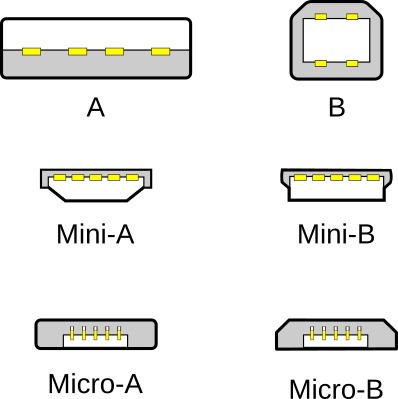
\includegraphics[width=0.28\textwidth]{usbconector}
	\caption{Tipos de conectores USB. Los tipo A deben ser usados en el extremo del Host y los tipo B hacia los periféricos\cite{USBHardwareWiki}}
	\label{fig:con}
\end{figure}

Cada uno de estos dispositivos diferentes, se inteconectan entre sí a través de cables y conductores específicos, diseñados en forma tal que no sea posible conectarlos en forma equivocada. Para cumplir con la norma, el Host debe tener siempre un zócalo compatible con conectores tipo A y los periféricos para enchufes de tipo B. Se observan las diferencias entre uno y otro en la Figura \ref{fig:con}
%		\section{Dispositivos USB}
%			\label{usb:dispo}
		\subsection{Dispositivos que componen un sistema USB}
			\label{usb:disp}
			Dentro de un sistema USB existen tres tipos diferentes de dispositivos: Host, Hubs y Funciones. Cada uno de ellos tiene asignado un rol específico dentro de la comunicación. Se detallan a continuación las tareas pertinentes a cada uno de ellos.\\

\subsection{Host USB}
	El Host es quien comanda las comunicaciones. Este dispositivo debe tener capacidades de memoria y procesamiento necesarias para almacenar y ejecutar el software de control. A su vez, necesita de hardware que le permita llevar un monitoreo y control de los eventos que suceden en el bus. Entre las tareas que debe llevar a cabo, se encuentran:
	
	\begin{itemize}
		\item Detectar la conexión y desconexión de dispositivos.
		\item Administrar el flujo de los comandos de control con los diferentes dispositivos.
		\item Administrar el flujo de la información entre él (Host) y los diferentes dispositivos.
		\item Llevar estadísticas de actividad y estado del bus.
		\item Proveer potencia a los dispositivos conectados, cuando estos así lo requieran.
	\end{itemize}
	
	Debido a que las tareas que ejecuta el Host requiere una cantidad de recursos de almacenamiento y procesamiento, es usual que el sea una PC la que lleve el rol. El Host es quien inicia la comunicación con las Funciones. Las Funciones, a su vez, responden a lo que fue solicitado por el Host, cuando él lo indique.\\
	
\subsection{Hubs USB}
	Un Hub USB tiene la función de proveer puertos al bus. El primer Hub esta incorporado en el Host y cada vez que se requiere más puertos a los cuales incorporar periféricos, se puede ir agregando a través de Hubs. Otra función importante es la de servir como interfaz entre dispositivos con diferentes velocidades, optimizando así el ancho de banda disponible para la comunicación.\\
	
\subsection{Funciones USB}
	La norma define como Función a todo aquel dispositivo que se conecta al bus y brinda al Host la capacidad de realizar una nueva tarea. Por ejemplo, un teclado otorga un método de entrada adicional, un mouse permite manejar un puntero de la interfaz gráfica, un parlante y un micrófono posibilitan la emisión y recepción de sonidos, respectivamente. Cada una de estas utilidades, compone una Función USB. A su vez, un dispositivo que brinda más de una capacidad es visto por el Host como Funciones separadas conectadas a través de un Hub. Por ejemplo, si se piensa en unos auriculares con micrófono, como los usados por una operadora en un centro de llamados, aunque se presenten integrados en un mismo producto y tengan un único puerto de conexión al bus, el Host los considera como dos Funciones separadas. Las Funciones, desde un punto de vista de software, son independientes unas de otras, por lo que cuando un programa, llamado cliente, necesita utilizar una de ellas, puede acceder a ésta directamente sin conocer cuantas y cuales funciones diferentes existen en el bus.\\
	
	Cada Función se compone de un conjunto de extremos. Un extremo es una porción de dispositivo identificable en forma unívoca\cite{USBspec}. Cada extremo tiene características definidas por el diseñador del sistema que deben estar adecuadas a los requerimientos de cada dispositivo. Los extremos tienen un solo sentido de comunicación y un tamaño máximo de mensaje a transmitir o recibir. Cuando se conecta al bus, un dispositivo debe enviar una descripción en donde consten sus extremos y las diferentes formas de configuración de cada uno, con el tipo de mensajes que soporta, el sentido de la comunicación, el tamaño, entre otros parámetros. Esta descripción se lleva a cabo través de lo que la norma llama descriptores.\\
	
	Todo dispositivo debe contener un extremo con dirección cero dedicado exclusivamente al control de la Función por parte del Host. Debe, como mínimo, poder comunicarse a velocidad completa, es decir, con una señal de \SI{12}{\mega\bit\per\second} y, a su vez, responder a los comandos de control básicos cómo adquirir la dirección, recibir la configuración y enviar los descriptores del dispositivo y sus diferentes configuraciones. Dependiendo de las diferentes requerimientos, el dispositivo puede incorporar otros extremos (15 de entrada y 15 de salida como máximo). Cada extremo no-cero tiene diferente latencia, acceso al bus, ancho de banda, manejo de errores, tamaño máximo de paquete soportado y dirección.\\
	
	
%	punto de vista lógico, cada periférico posee canales únicos de comunicación con el host, llamados tuberías ({\it pipes} en el idioma inglés de la norma). Existen dos tipos de tuberías, las de control, por donde circulan mensajes propios del protocolo y sirven para la administración, configuración y gestión de las comunicaciones ; y las tuberías de ``chorro'' ({\it stream}) a través de las cuales circulan los mensajes con la información que se desea transmitir de un dispositivo a otro. El final de la tubería se llama extremo ({\it endpoint}) en el periférico y conectan cada extremo a un buffer en el host. Los periféricos poseen uno o más extremos. Cada extremo de un periférico, posee un tipo de transferencia asociado con una dirección de la información determinada. Esto quiere decir que un dispositivo de entrada y salida, debe poseer al menos dos extremos lógicos diferentes, uno para enviar datos al host y otro para recibirlos. Los tipos de transferencia, a su vez, determinan el ancho de bus asignado por el protocolo, la latencia, la tolerancia a errores en los datos enviados y el tamaño de los paquetes a enviar.\\
	
		\subsection{Paquetes USB}
			\label{usb:pkt}
			%TODO descripcion de paquetes y campos de los paquetes
Los dispositivos transmiten información a través del bus con un formato particular, establecido por el protocolo que dicta la norma USB. Cada \SI{1}{\milli\second}, el Host debe emitir una señal de sincronismo. El intervalo que transcurre entre una señal y la siguiente, se denomina cuadro. El Host asigna una porción de cuadro a cada uno de los dispositivos, asignando ancho de banda y tiempos de retardo a cada uno, según los requerimientos. A su vez, en comunicaciones de Alta-Velocidad, cada cuadro se subdivide en 8 microcuadros de \SI{125}{\micro\second} cada uno. Los fragmentos de información que envían los dispositivo mientras transcurre un cuadro, se denominan paquetes. Un paquete está compuesto por diferentes campos. El sistema reconoce cada campo, decodifica su información e identifica cada paquete, su emisor, el tipo de datos que envía, el sentido de circulación. Luego, corrobora que los datos transmitidos llegaron a destino en forma satisfactoria. 

\subsection{Campos de paquetes}
	Existe un número finito de campos y todos pueden resumirse en el presente documento. Sin embargo, se detallan a continuación los que el autor considera más relevantes para el objetivo de este trabajo, quedando de lado algunos comandos, por ejemplo, inherentes a los hubs que conectan dispositivos de diferentes velocidades.

	\subsubsection*{Identificador de paquete}
		El campo identificador de paquete (PID del ingles {\it Packet Identifier}) le da a conocer a los distintos dispositivos el tipo de información que contiene el paquete. Por ejemplo, indica si el Host solicita envío o recibo de datos, si envía un comando o si un dispositivo está transmitiendo los datos. Se compone de un campo de 8 bits, de los cuales 4 corresponden al identificador propiamente dicho y los otros cuatro son el complemento a uno de los mismos datos, permitiendo corroborar que no hubo una pérdida de información.%\\
		
		Existen 4 tipos de PID: Token, que antecede a cualquier transmisión y es emitido por el host; Data, indica paquetes que contienen datos transmitidos; Handshake, a través del cual los componentes del sistema se enteran si la comunicación fue efectiva o no y Special, cuya función no es de interés para este trabajo.%\\
	
		A su vez, los PID Token se dividen en 4 tipos: IN, para indicar que se va a realizar una envío de datos desde un extremo al Host; OUT, antecede a una transmisión de datos en el sentido contrario, es decir del Host a un extremo; SETUP, que señala una secuencia de comandos y SOF (del inglés {Start of Frame)} que emite una señal de inicio de cuadro, utilizada para sincronismo y control.%\\
	
		Dentro de los PID Data, solo existen diferentes etiquetas que se usan dependiendo del tipo de transmisión. Los PID de Handshake contienen 4 mensajes diferentes: ACK para indicar que el mensaje fue recibido satisfactoriamente y NAK señala que no se pudo enviar o recibir, STALL significa que el extremo se detuvo y NYET de cuenta sobre demoras en la respuesta del receptor.
	
	\subsubsection*{Dirección}
		El campo de Dirección señala cuál es la Función que debe responder o recibir alguna directiva emitida por el host. A su vez, se divide en dos subcampos: uno que indica un dispositivo y la segunda que señala el extremo específico con el cual desea comunicarse.

	\subsubsection*{Datos}
		Es el campo que contiene la información útil transferida. Puede tener un largo de hasta 1024 bytes. Cada byte enviado se ordena con el bit menos significativo (LSb del inglés {\it Less Significative bit}) primero y el bit mas significativo (MSb por sus siglas en inglés) al final.

	\subsubsection*{Chequeos de redundancia cíclica}
		El campo de chequeo de redundancia cíclica (CRC) contiene verificadores para corroborar que no hubo pérdida de información. Dependiendo de que tipo de paquete se esté transmitiendo, el CRC puede tener 5 o 16 bits. 
%		Los códigos generadores son representados por las ecuaciones 2.1 y 2.2 respectivamente:
%	
%		\begin{center}
%			\begin{align}
%				G(X)&=X^5+X^2+1\\
%				G(X)&=X^{16}+X^{15}+X^2+1
%			\end{align}
%		\end{center}
	
\subsection{Formato de paquetes}
	Cada uno de los paquetes que intervienen en la comunicación USB utilizan diferentes tipos de campos, dando lugar a distintos tipos de paquetes. La figura \ref{fig:paq} muestra como se conforman algunos de ellos.%\\ 

	\begin{figure}
		\centering
		\begin{tikzpicture}[scale=.8,>=latex]
			\begin{scope}
				\begin{scope}[transform shape,node distance=.15]
					\node[pid]	(pidtok)	{PID: \\SETUP};
					\node[dir]	(adtok)	[right=of pidtok]	{Dir. \\Disp.};
					\node[dir]	(eptok)	[right=of adtok]	{Extr.};
					\node[crc]	(crc5)	[right=of eptok]	{C\\R\\C\\5};
				\end{scope}
				\begin{scope}
					\node[exterior,minimum size=0,inner sep=1,fit=(adtok)(eptok)](tokad){};
					\node[below=.01 of tokad.south,align=center,transform shape] (texttok){Paquete\\Token};
					\node[rounded corners, exterior,inner sep=1,fit=(pidtok)(tokad)(crc5)(texttok)](pkttok){};
				\end{scope}
				\begin{scope}[transform shape,node distance=.15]
					\node[pid,node distance=.4]	(piddat)	[right=of crc5]{PID: \\DATA};
					\node[data]	(data)	[right=of piddat]	{Datos\\útiles};
					\node[crc]	(crc16)	[right=of data]	{C\\R\\C\\1\\6};
				\end{scope}
				\begin{scope}
					\node[below=.01 of data.south,align=center,transform shape] (textdat){Paquete\\de Datos};
					\node[rounded corners,exterior,inner sep=2,fit=(piddat)(data)(crc16)(textdat)]{};
				\end{scope}
				\begin{scope}[transform shape,node distance=.15]
					\node[pid,node distance=1.3]	(hspid)	[right=of crc16]%.north east,anchor=south east]
						{PID Hs};
				\end{scope}
				\begin{scope}
					\node[below=.01 of hspid.south,align=center,transform shape] (texths){Paquete\\de Handshake};
					\node[rounded corners,exterior,inner sep=2,fit=(hspid)(texths)]{};
				\end{scope}
			\end{scope}
			\end{tikzpicture}
		\caption{Formatos de paquetes}
		\label{fig:paq}
	\end{figure}	

	Un paquete de tipo Token está conformado por los campos PID, Dirección y CRC-5 (CRC de 5 bits). Un paquete Token que indica SOF en su campo PID, lleva un formato un poco diferente. En lugar de la dirección, se envía un contador de 11 bits que señala la cantidad de cuadros que han transcurrido desde la puesta en marcha del sistema, seguido de un código CRC-5.%\\
		
	Cada \SI{1}{\milli\second} el host transmite un SOF e incrementar el contador de cuadros. En sistemas USB 2.0 de Alta velocidad, además, se transmiten 8 subcuadros de \SI{125}{\micro\second} por cada cuadro. Cada uno de estos subcuadros inicia con un paquete SOF. Sin embargo, el host no actualizará el número de cuadros hasta pasado \SI{1}{\milli\second}.%\\
		
	El paquete de datos iniciará con un PID que indique que es un paquete de este tipo, luego enviará los datos desde el LSb hasa el MSb y, finalmente, enviará un código CRC-16 (CRC de 16 bits de longitud).%\\
		
	Los paquetes de tipo Handshake (Hs) solo envía un PID con información sobre si el mensaje fue recibido en forma correcta o no.
		\subsection{Tipos de Transferencias}
			\label{usb:xfer}
			Cada extremo presente en un dispositivo USB, puede estar configurado, en simultaneo, con un solo tipo de transferencias. Es importante, para el diseñador del dispositivo, entender y seleccionar el tipo de transferencia adecuada para cada uso debido a que, de ello depende las características que poseerán las comunicaciones que se efectúen.\\

Existen cuatro tipos de transferencias definidas por la norma USB: Transferencias de Control, transferencias en, transferencias isocrónicas y transferencias de interrupción. Cada una de ellas tiene un propósito y características diferentes, las que se detallan a continuación.\\

\subsection{Transferencias de control}
	Las transferencias de control son utilizadas por el host para comunicaciones de configurar, emitir comandos y conocer el estado de los distintos dispositivos acoplados al bus. Se caracteríza por ser una comunicación de rafagas, es decir, de corta duración y de alta prioridad, no periódica de tipo, pregunta-respuesta, es decir, el host solicita y el dipositivo responde en función a la solicitud.\\
	
	Habitualmente, este tipo de comunicaciones se utiliza solamente para emitir comandos hacia los dispositivos, o bien, para conocer su estado.\\
	
\subsection{Transferencias en masa}
	Este tipo de transferencias son usadas para transferir paquetes grandes en forma ráfagas no periódicas. Su utilidad consiste en que permite aprovechar al máximo cualquier espacio de ancho de banda disponible.\\
	
	Gracias al sistema de chequeo de errores, es posible solicitar retransmisiones, de forma de asegurar la integridad del mensaje transmitido. Esta transferencia es ideal para comunicar paquetes de datos que no son crítico en tiempo pero que requieren una comunicación fidedigna.\\

\subsection{Transferencias isocrónicas}
	Este tipo de transferencias son periódicas y continuas entre el host y los dispositivos. Son muy interesantes para información que pierde validez cuando no es entregada en un tiempo establecido.\\
	
	Debido a la criticidad del tiempo de entrega de los datos comunicacdos con este método, no se prevee una retransmisión de los datos enviados por este sistema.\\
	
\subsection{Transferencias de interrupción}
	Cuando se requiere de una comunicación con latencia asegurada pero con baja probabilidad de eventos, el tipo de transferencia óptimo para utilizar, son las transferencias de interrupción.
		\subsection{Descriptores}
			\label{usb:dscr}
			%INTENTO 2
%Un mismo dispositivo puede tener multiples configuraciones conforme a la disponibilidad del sistema que lo aloja, la disponibilidad de ancho de banda, entre otras características. Incluso, dependiendo del uso del dispositivo, este puede operar a diferentes velocidades y requerir diferentes tipos de ancho de banda.
%
%El dispositivo puede tener uno o más extremos, los cuales pueden designarse en una o mas interfaces. A su vez, las interfaces se agrupan en configuraciones y se subdividen en alternativas.Estas múltiples configuraciones, deben ser comunicadas al host a traves de un tipo especial de mensajes, con estructura y formato establecido, denominado descriptores.

%INTENTO 3
Cuando un dispositivo es conectado al bus, debe informar sus características al Host a través de descriptores. Un descriptor es un estructura de datos con formato definido. De esta forma, el sistema conoce las diferentes configuraciones que puede tener cada una de las Funciones conectadas. El conocimiento detallado de estos descriptores por parte de los diseñadores de dispositivos, facilita luego la tarea de selección de cada uno de los atributos que tendrá, como así también, la elaboración de software cliente en la \acrshort{pc}.%\\

Cada uno de los descriptores comienzan con su longitud en bytes y el tipo de descriptor que se está enviando. En orden jerárquico, se utilizan categorías de descriptores que van desde los atributos generales a los particulares. En primer lugar, se envía el descriptor DEVICE que informa la versión de la norma USB que cumple el dispositivo, un número que identifica al fabricante y otro que corresponde al producto, es decir al dispositivo. Esto puede ser utilizado por el Host para ejecutar el software de control adecuado para comunicarse con el dispositivo. A su vez, comunica la cantidad de posibles configuraciones. Luego, si el dispositivo cumple con la norma 2.0 (o más moderna) envía un descriptor de tipo DEVICE\_QUALIFIER con información sobre otras velocidades de comunicación soportadas.%\\

El protocolo \acrshort{usb} diferencia una configuración de otra dependiendo de las necesidades de energía. Un dispositivo podría operar conectado a una fuente de energía externa, o bien, ser alimentado por el mismo bus. Si las potencias de la fuente y del bus son diferentes, podrían verse limitadas las utilidades que ejecutaría la Función. Entonces, cuando el dispositivo funcione con la fuente podría tener una configuración pero cuando se desconecta, deberá informar esta situación al Host, indicando que se debe cambiar la configuración. Esta comunicación se lleva a cabo a través del descriptor de tipo CONFIGURATION. Debe haber tantos descriptores de este tipo como se indicó en el descriptor DEVICE.%\\

Debido a que cada configuración puede tener diferentes limitaciones en sus funciones dependiendo de la potencia que consuma, se establece que cada configuración tenga a su vez diferentes interfaces. La cantidad de interfaces que tiene una configuración, también debe estar informada en el descriptor CONFIGURATION.%\\

Una interfaz puede verse como el conjunto de extremos que son utilizados por un dispositivo para realizar una función específica. Por ejemplo, se podría pensar en una impresora multifunción. Se puede tener una interfaz para la función de impresión y otra para la de escaneo. A su vez, cada interfaz puede variar el ancho de banda requerido a través de una característica denominada \textit{AlternateSettings}. Las interfaces y sus diferentes alternativas, se comunican al Host a través del descriptor de tipo INTERFACE.%\\

A su vez, un extremo define la dirección de la comunicación, es decir, si es desde o hacia el Host, un tipo de transferencia, si la comunicación es sincrónica o no, el tamaño máximo de paquete y el ancho de banda necesario. Los extremos se describen a través del descriptor ENDPOINT.%\\

En resumen, la comunicación entre los dispositivos y el Host se efectúa a través de los extremos. Los extremos, a su vez, se agrupan en interfaces y un grupo de interfaces conforman una configuración. Una característica a tener en cuenta es que un dispositivo puede tener diferentes interfaces activas a la vez y las interfaces pueden cambiar durante la operación de características alternativas (\textit{AlternateSettings}). Sin embargo, al cambiar de configuración, todos los extremos y las interfaces son desactivadas.%\\

También existe un tipo de descriptores, denominados STRING, que sirven para colocar a cada uno de los atributos una forma legible por el usuario, aunque puede no ser utilizada. 
%INTENTO 1
%Para ello, este último inicia una transferencia de control, requiriendo los atributos de la nueva función. Este informe, se realiza a través de un tipo especial de mensajes, con una estructura y formato determinado, que se denominan descriptores. Los descriptores son muy importantes porque es a través de ellos que el host y los dispositivos determinan las formas en que va a operar y comunicarse una función determinada. Existen siete descriptores USB standard:

%\begin{itemize}
%	\item Device: contiene información sobre, la versión de USB que cumple, la clase de dispositivo conectada, el fabricante, el número de identificación del producto, numero de serie y la cantidad de diferentes configuraciones que posee.
%	\item Device\_Qualifier: En dispositivos que son capaces de operar a Alta Velocidad, informa sobre atributos que cambian cuando opera a otra velocidad.
%	\item Configuration: Contiene información sobre la configuración específica del dispositivo. Cada descriptor de dispositivos informa el número de interfaces diferentes que contiene esa configuración. Cada interfaz, a su vez, puede contener distinta cantidad de extremos, conforme a la necesidad.
%	\item Other\_Speed\_Configuration: indica configuraciones de un dispositivo que puede operar a alta velocidad cuando está operando a otra velocidad posible.
%	\item Interface: 
%	\item Endpoint
%	\item String
%
%\end{itemize}%Los descriptores dan cuenta al host de que clase de dispositivo se conecta, cuales son sus posibles configuraciones, que interfaces tiene cada una de ellas, las velocidades a las que puede operar, los extremos que posee, etc. Existen varios tipos de descriptores que informan diferentes atributos o características. Lo que tienen en común unos y otros, es que al momento de la conexión al bus, estos deben ser informados al host.\\



%		\section{Sumario del Capítulo}
%		\label{usb:sum}
%		En el presente capítulo se desarrolló y justificó la elección del controlador FX2LP como nexo entre la FPGA y la PC, brindando la conexión USB necesaria. Luego, se explicaron algunos componentes de la arquitectura implementada por Cypress a fin de proveer la comunicación USB. Finalmente, se detalló paso a paso cada uno de los componentes configurados, como así también el código desarrollado para dicho fin.

Además, se mostraron algunos detalles del framework provisto por Cypress y los encabezados necesarios para su utilización y se explicitaron los descriptores a través de los cuales se le informa al sistema las características de la comunicación que se implementa.
	\section{Objetivos}
		\label{int:obj}
		\subsection{Objetivo Principal}
	El objetivo del presente trabajo es obtener una comunicación USB 2.0 de alta velocidad entre una PC y un FPGA.%\\
	
	Esta comunicación debe realizarse y documentarse de forma tal que pueda ser usado posteriormente en aplicaciones científicas desarrolladas con FPGA's.
	
\subsection{Objetivos Particulares}
	Para la consecución del objetivo general, se deben cumplir los siguientes objetivos particulares:
	
	\begin{itemize}
		\item Comprender el funcionamiento del protocolo USB.
		\item Seleccionar los componentes a utilizar.
		\item Configurar los componentes seleccionados.
		\item Desarrollar un núcleo en VHDL que sirva de interfaz.
		\item Diseñar e implementar la interconexión de los componentes seleccionados.
		\item Verificar el sistema desarrollado.
		\item Desarrollar un documento que explique el modo de uso del código VHDL utilizado.
	\end{itemize}
	\section{Estructura del Informe}
		\label{int:est}
		El presente informe se divide en 2 bloques principales: uno referido al desarrollo del sistema y el siguiente a su forma de uso y verificación.

Dentro del bloque referido al desarrollo del sistema, se encuentran los primeros 5 capítulos:

\begin{enumerate}
	\item {\bf \nameref{cap:int}:} En este capítulo se intenta exponer lo que motiva el presente trabajo, la propuesta que da solución a la motivación, el objetivo y alcance que el trabajo busca y la estructura del mismo. Se brindan, además, conceptos importantes de la norma USB que son significativos para los objetivos de este trabajo.
	\item {\bf \nameref{cap:mats}:} Se describe aquí todas las herramientas de las que se vale este trabajo para cumplir con os objetivos propuestos.
	\item {\bf \nameref{cap:cy}:} Se presenta la arquitectura, configuración y código desarrollado para el presente trabajo, como así también las herramientas específicas provistas por el fabricante, que facilitan el desarrollo. 
	\item {\bf \nameref{cap:fpga}:} Este capítulo detalla lo desarrollado para implementar la comunicación entre la FPGA y la interfaz. Se expone una máquina de estados descrita en VHDL y sintetizada en FPGA. También se describe un circuito impreso realizado para conectar ambas partes.
	\item {\bf \nameref{cap:verif}:} Se desarrolla las tareas desarrolladas a fin de realizar las depuraciones del sistema y la verificación del cumplimiento de las especificaciones.
\end{enumerate}
	\section{Sumario del capítulo} 
		\label{int:res}
		En el presente capítulo se expuso la necesidad de elaborar un sistema de comunicación que permita la transferencia de datos entre una \acrshort{pc} y un \acrshort{fpga} para ser utilizados por desarrollos científicos implementados con este último dispositivo.

Se propuso utilizar una interfaz comercial como intermediario los dos dispositivos y se brindó una justificación del empleo del protocolo \acrshort{usb} 2.0 de alta velocidad para una comunicación óptima que satisfaga los requerimientos.

Además, se repasaron algunos conceptos importantes inherentes a la versión 2.0 de la norma \acrshort{usb}.

Se presentaron también los objetivos formales del trabajo y la estructura del presente informe.
		
%  %for looking file porpuse.. comment before compile
%	Un carpintero desea medir la distancia de una barra de madera que luego será, tal vez, la altura de las patas de una futura mesa. Para ello, utiliza una cinta métrica, compuesta de una cinta metálica que posee una escala graduada. Sabe entonces que la barra mide la distancia que coincide con la distancia de la cinta graduada.\\

Un panadero desea medir cuanto pesa la harina que debe para poder amasar. Entonces, la coloca en una balanza y observa cuanto marca su indicador. Así conoce que la masa de la harina es equivalente a la fracción de medida que indica la balanza.\\

Un atleta desea conocer cuanto demora en correr un trayecto que posee \SI{1}{\kilo\metro}. Por esto, registra el valor que indica su reloj al principio del recorrido y cuando alcanza el final observa nuevamente el artefacto. Luego de esto, calcula la diferencia entre el valor final y el inicial, conociendo cuanto tiempo le tomó realizar su travesía.\\

En los tres casos anteriores, tanto el carpintero, como el panadero y el atleta desconocen algo y necesitan cambiar su estado con respecto a esa incertidumbre. Por ello recurren a diferentes objetos, a fin de obtener conocimiento a partir de ellos. Sin embargo, estos objetos, por si mismos, no otorgan información, sino más bien otorgan un dato, que comparado y contrastado con otros datos, se traducen en conocimiento.\\

La información es el resultado de ordenar y procesar un conjunto de datos, de forma tal que permitan cambiar el estado de conocimiento sobre un asunto determinado. En el caso del carpintero, compara el tamaño de las patas de la mesa con una cinta metlálica, que a su vez, posee registrada su distancia en función de algún patrón de metrología, establecido por convención. Esto quiere decir que el dato 1, la longitud del patron, junto al dato 2, escala graduada de la cinta, más el dato 3, la longitud de la cinta métrica, permiten al carpintero cambiar su estado de desconocido a conocido, con respecto a la longitud del trozo de madera, a través de la información proporcionada por el conjunto de datos.\\

Se puede realizar el mismo análisis con respecto a la balanza del panadero, considerando un peso patrón, un desplazamiento y una escala graduada o una señal eléctrica emitida por una celda de carga deformada un porcentaje de su capacidad, registrada previamente por su fabricante conforme a pesos patrones, y un circuito adaptador que transforma esa señal electrica en un valor numérico mostrado en un indicador.\\

El atleta compara las posiciones y los desplazamientos de las agujas de su reloj, previamente calibrado para que dé una vuelta por cada minuto en una aguja, otra aguja que dé una vuelta por hora y la tercera una vez cada 12 horas. Además, es probable que él haya ajustado la hora que indica el reloj para que otorgue un horario idéntico al de referencia, establecido por convención.\\

En todos los casos, se posee una gran cantidad de datos que, ordenados, procesados y comparados otorgan al usuario un valor útil, ya sea una longitud, una masa, un tiempo o cualquiera sea la variable física que se desee conocer.\\

La ciencia es un conjunto de técnicas y procedimientos que, a través del método científico, busca adquirir, descubrir y/o desarrollar nuevo conocimiento. Se desprende entonces, que la ciencia produce, de forma fundamental, información que luego es transformada en conocimiento. Cuando hablamos de ciencia, hablamos de una gran gama de objetos de estudio, sujeto a través del cuál se clasifican, en la mayoría de los casos, las ciencias: las Ciencias Sociales estudian las relaciones humanas, las Ciencias Naturales estudian objetos que se encuentran en la naturaleza, las Ciencias de la Tierra se enfocan en una rama más particular de la naturaleza, como lo son los minerales, la superficie terrestre, etc; y siguiendo así se puede encontrar un sinnuméro se ciencias. Sin embargo, toda ciencia necesita, para su correcta producción científica, adquirir una gran cantidad de datos que luego será nordenados, procesados y transformados en información y conocimiento.\\

La incorporación de una herramienta especialmente diseñada para el procesamiento de datos, como lo es la computadora, permite manejar un numero cada vez creciente de información.
Es por eso que se encuentra en desarrollo un gran número de sensores y dispositivos que permitan obtener cada vez más datos.\\

En este sentido, una de los desarrollo que se encuentran en boga es el sensores que adquieran imágenes. Como ejemplos podemos encontrar, entre muchos otros, el desarrollo de sensores de radiación[1], ultrasonografía[2], telescopía de objetos cercanos[3], imagenes de distancia[4].





[1][https://ieeexplore.ieee.org/abstract/document/8214376]
[2][http://www.idr.iitkgp.ac.in/jspui/bitstream/123456789/9068/1/NB15975_Abstract.pdf]
[3][https://ieeexplore.ieee.org/abstract/document/8396725]
[4][https://www.sciencedirect.com/science/article/pii/S0030402617316029]




El mundo actual, en el que vivimos inmersos, demanda y consume volumenes cada vez más grandes de información. Con solo hacer una rapida miradad en diarios, incluso no especilizados, se observa la importancia que poseen las ciencias y disciplinas que manejas la informacion, aquellas areas agrupadas dentro del conjunto Técnico de la Información y la Comunicación, o más ocnocido por sus siglas, TIC's.

Internet de las cosas , Big Data, Inteligencia Artificial, Redes Neuronales, Robótica, Domótica, entre otras, son areas en las que los datos y la información es abultada y su correcto manejo es sumamente complejo e importante. Además, ninguna de las actividades científicas, puede escapar de esta gran demanda mundial de información.

La información es un conjunto de datos ordenados y procesados de forma tal que permita al que lo lea que eleve su nivel de conocimiento sobre un determinado tema. Es decir que, para que exista información, en primer lugar tenemos que tener datos, de forma tal que podamos luego procesarlos y obtener realmente información de llos.

Como ejemplo de esto, podemos citar simplemente el acto de medir la presión dentro de un tubo de gas. Sería normal pensar en que, teniendo este objetivo en mente, simplemente coloquemos un manómetro en la salida del tubo. El manómetro es un artefacto que posee una varilla 





El mundo, durante la era de la información, nos exige producir y consumir cada vez más y más información. En cada aspecto social dela vida de la persona se pueden encontrar ejemplos claros de esto.\\

Bajo un punto de vista social nos vemos bombardeados por información. Los 'influencers' que se mueven a traves de Facebook, Twiter, Instagram, Snapchat, Linkedin, Youtube, etc, necesitan para estar a la moda, producir constantemente material y que ese material sea consumido por alguien que este demandando esa información.

En el area de econimía y finanzas existen cada vez más robots que extraen información de las diferentes bolsas, periodicos, bancos, industrias y donde se ocurra que pueda haber información útil, para tomar mejores decisiones que, por supuesto, también ejecutan los robots.

En el comercio, desde las tiendas de supermercado hasta las tiendas digitales que trabajan solo a través de internet están constantemente recabando datos y procesandolos a din de diseñar estrategias que permitan ofrecer productos que se adapten mejor a lo que busca el cliente y de esa forma lograr vender mayores volumenes.

La industria cuenta cada vez más con multiplicidad de posibilidades basadas en sensores que adquieren grandes cantidades de datos que son almacenadas y procesadas, muchas vecen 'en línea' o 'al instante', de forma tal de encontrar mejores procesos o ejecutar nuevas tareas, como por ejemplo la industria automotriz, enfocada cada vez más en autos que puedan manipular todo el entorno y ser totalmente autónomos de un conductor.
La industria espacial y satelital dotan a sus equipos de mayores sensores y mayores flujos de datos. La industria médica brinda cada vez más posibilidades de diagnóstico a traves de nuevas técnicas y formas de adquisición de imágenes.

A todo esto, la ciencia y el desarrollo de nuevas aplicaciones y equipos, no son indiferente. Cada vez se encuentran más innovaciones y desarrollos de nuevos sensores que adquieren flujos de información crecientes. La toma de imagenes se ha vuelto una herramienta clave para la investigación en diversas areas, tales como la biología, la ciencia de materiales, las ciencias nucleares, las ciencias de la tierra, etc.

Las redes sociales son un ejemplo de esto, pero esto se observa en la industria, la economía, las finanzas e incluso hasta en la casa.



[1] file:///home/lechuzin/Facultad/Trabajo%20Final/lechuzing/docs/bibliografia/The-Rise-of-the-Network-Society-With-a-New-Preface-Volume-I-The-Information-Age-Economy-Society-and-Culture-Information-Age-Series-.pdf
%	El Bus Serial Universal, o USB por sus siglas en inglés, es un sistema de comunicación diseñado durante los años 90 por seis fabricantes vinculados a la industria informáticas, Compaq, Intel, Microsoft, Hewlett-Packard, Lucent, NEC y Philips, con la idea de proveer a su negocio de un sistema que permita la conexión de PCs con teléfonos y periféricos con un formato estándar, fácil de usar y que permita la compatibilidad entre los distintos fabricantes.\\

Hasta ese momento, el gran ecosistema de periféricos, sumado a los nuevos avances y desarrollos, hacia muy compleja la interoperatividad de todos ellos. Cada uno de los fabricantes desarrollaba componentes con características, tales como fichas, niveles de tensión, velocidades, drivers, lo cuál dificultaba al usuario estar al día y poder utilizar cada componente que compraba. Esto también complicaba a las mismas empresas productoras, por que la introducción de un nuevo sistema requería de mucho soporte extra para poder conectar todo lo ya existente.\\

Todo esto, quedó saldado con el aparición de la norma USB que, gracias a la gran cuota de mercado de sus desarrolladores, fue adoptado en forma rápida y se transformó en la especificación por defecto a la hora de seleccionar un protocolo. Al punto tal esto se cumplió que hoy, más de 20 años después, es muy difícil encontrar PC's con otro tipo de puertos, salvo que, en el momento de su compra, se solicite especialmente un puerto determinado. Así, cualquier PC nueva disponible en el mercado debe poseer puertos USB para la conexión de los periféricos.\\

El diseño de la norma USB busca resolver tres problemáticas interreacionadas, que son: La conexión de teléfonos con las PC, la facilidad de uso, es decir, que el usuario solo conecte su dispositvo y pueda utilizarlo, y la expansión en la cantidad de puertos disponibles para conectar periféricos\cite{USBspec}. Para satisfacer estas tres demandas, la norma USB 2.0 busca alcanzar un conjunto de metas que apuntan a la facilidad del uso, la compatibilidad entre versiones diferentes de la misma tecnología, la robustez en el flujo de datos, y la convivencia de diferentes configuraciones temporales en único bus, provistos de una interfaz estándar, ancho de banda que soporte comunicaciones audiovisuales de calidad aceptable y un bajo coste.\\

El presente capitulo intenta ser un breve resumen con los aspectos más relevantes de la norma en cuanto a su composición física, su topología, los dispositivos que intervienen, la importancia de los mismos y como los datos son transmitidos desde y hacia una PC.\\

%	Desde el punto de vista técnico, el protocolo USB es un sistema del tipo maestro-esclavo, donde el maestro, denominado {\it HOST}, debe ser necesariamente una PC (o un dispositivo con software y hardware capaces de incorporar los drivers necesarios) y cualquier periférico a ella acoplada será un esclavo\cite{USBspec}.\\
%	
%	Para describirlo es conveniente diferenciar tres partes. Una capa física, en donde se definen los componentes que intervienen, una capa de protocolo, en donde se define el formato, el marco en el que son enviados los paquetes, como se direccionan y como se comunican entre sí, y una parte lógica, en donde cada componente es visto solamente como un extremo y define como fluyen los datos desde un extremo hacia la PC y viceversa.\\
%	
%	\subsection{Capa física}
%		
%	\begin{figure}[!ht]
%		\centering
%		\begin{tikzpicture}[scale=1.2\textwidth/\paperwidth,>=latex]
%			\begin{scope}
%				\begin{scope}[transform shape,node distance=2,grow=right,sibling distance=80, level distance=30]
%					\node[draw=black] (host) {\it HOST}
%						child {node[hub] (root) {Raiz} edge from parent[level distance=70,<->]
%							child{node[hub](hub){HUB} edge from parent [<->,sibling distance=35,level distance=50]
%								child {node	[dev]	(out){Función} edge from parent [<-]}
%								child {node	[dev]	(in){Función} edge from parent [->]}
%								child {node (text) {Dispositivo compuesto} edge from parent [draw=black!0]}
%							}
%							child{node[dev]{Función} edge from parent [->]}
%							child{node[dev]{Función} edge from parent [<-]}
%						};
%				\end{scope}
%				\begin{scope}
%					\node[draw=black,rounded corners, dashed, fit=(hub)(out)(in)(text)]	(comp)	{};
%				\end{scope}
%			\end{scope}
%		\end{tikzpicture}
%		\caption{Topología de un sistema USB}
%		\label{fig:arqusb}
%	\end{figure}
%		
%	En esta sección no se describirán los detalles de las conexiones eléctricas ni mecánicas a las que se refieren las especificaciones de la norma USB debido a dos cuestiones fundamentales. Una de ellas es que toda esta sección de la norma está resuelta ya por los fabricantes de la interfaz que se utiliza en este trabajo. A su vez, maneja todas las señales, arma y desarma los paquetes que salen hacia la PC y que llegan de ella respectivamente. Por otro lado, no es el objetivo de este trabajo adentrarse en esos detalles. Gracias a la extensión de este tipo de comunicación existen una gran cantidad de fabricantes en el mercado que fabrican cada uno de los componentes, ya sean, cables, conectores en todas sus versiones, adaptadores de un tipo de estos, su costo es despreciable con respecto a cualquier tipo de desarrollo en ese sentido y son de una muy buena calidad, es decir que todos cumplen con lo que la norma establece. Sí, se describen los dispositivos físicos y su categoría, según la norma, en función del rol que cumplen.\\
%	
%	La comunicación USB posee una topología maestro-esclavo. Es decir, existe un dispositivo que dirige todas las transferencias de datos y otros que responden a sus directivas. Por esto, el elemento central de cualquier comunicación USB es el {\it HOST} (director o anfitrión, por su traducción de la voz inglesa). Él es el que posee el {\it Host USB Controller}\cite{USBspec}. Esto quiere decir que tiene la capacidad de registrar los dispositivos acoplados, asignarles dirección, colocar los paquetes de salida y/o llegada en sus respectivas listas y servilos a los procesos que utilizan esta comunicación. Además, el {\it HOST} se encarga de enviar los tokens a todos los periféricos, con la dirección del dispositivo, el sentido de la comunicación, el tipo de transferencia que se espera y todas las acciones de control que el sistema requiera. En la mayoría de los casos, el {\it HOST} es una PC, auqnue también puede ser cualquier dispositivos  ``inteligente'' como un smartphone.\\
%	
%	En el otro extremo de la comunicación, se encuentran lo que la norma denomina {\it funciones}\cite{USBspec}. Las {\it funciones} son todos los periféricos que actúan como fuente o sumidero de información. Es decir, en caso de periféricos de entrada, serán una fuente de datos hacia el {\it HOST}. Si los periféricos son de salida, serán un sumidero de la información que proporciona la PC. Los casos de periféricos de entrada/salida, se denominan {\it dispositivos compuestos}.\\
%		
%	Existe también, a los fines de la norma,un elemento intermedio, denominado {\it HUB} (concentrador o distribuidor, según la traducción del inglés). Este dispositivo se encarga de conectar dos o más {\it funciones}, ya sea de entrada o salida, de recibir y enviar las direcciones y de regenerar las señales que el {\it HOST} envía y deben ser recibidas por las {\it funciones}.\\
%	
%	La Figura \ref{fig:arqusb} muestra la topología típica de un sistema USB. En ella, se observa el {\it HOST} como un rectángulo, las {\it funciones} como rectángulos con los bordes redondeados y los distribuidores como círculos. Se puede notar que el {\it HOST} posee un distribuidor propio llamado {\it Raiz} en el cual se conectan todos las {\it funciones} y distribuidores. Cada {\it Función}posee una única dirección. Pueden existir dispositivos que posean funciones diversas con un mismo encapsulado, como por ejemplo un auricular que tenga micrófono incorporado. Este dispositivo, tendrá un {\it HUB} que concatena dos {\it funiones} diferentes.\\
%	
%	\subsection{Capa lógica}
%	Desde el punto de vista lógico, cada dispositivo es visto por el {\it HOST} como un extremo (EP, del inglés, {\it endpoint}) independiente, que posee solo un modo de comunicación, es decir, el protocolo se comunicara solo por un tipo de transferencia y en un único sentido con cada {\it EP}. En otras palabras, USB registra un periférico de entrada/salida como un {\it EP} de entrada y otro de salida en forma independiente.\\
%	
%	Esta independencia brinda la posibilidad de configurar cada extremo de forma diferente y obtener el ancho de banda necesario para la subida y bajada de datos, los tiempos de acceso al bus, la dirección y todo lo relacionado a los modos de comunicación conforme a los requerimientos.\\
%	
%	El protocolo entiende que entre le {\it HOST} y cada uno de los extremos existe un tubo (la norma en ingles habla de {\it pipes}) en donde la información es colocada y transferida. Luego, cada tubo posee la configuración establecida por el controlador del {\it HOST} y se comunica con cada {\it EP} por medio de estos tubos. A los fines del usuario, esto es lo importante, por cuanto se solicita acceso al bus y define en que buffer va a contener los datos a enviar o transmitir y el protocolo se encarga de el empaquetado, el armado de los cuadros, el acceso el bus y el posterior envío de datos.\\
%	
%	\subsection{Capa de protocolo}
%	En la capa de protocolo, la especificación de la norma detalla cómo se compone un cuadro y cómo deben ser estructurados los paquetes para que sean efectivamente enviados a través del sistema. Cada mensaje que se intercambia por el bus se denomina paquete. Cada paquete puede poseer hasta cinco campos, dependiendo del tipo de paquete que sea enviado a través del sistema y de quien sea el remitente. A su vez, cada paquete comienza con una señal de sincronismo ({\it SYNC}) y un Comienzo de Paquete (SOP de {\it Start-of-Packet}), y terminan con una señal de Fin de Paquete (EOP por {\it End-of-Packet}).\\
%	
%	Por otra parte, los paquetes está temporalmente encapsulados en cuadros. Cada cuadro posee un Comienzo de Cuadro (SOF, {\it Start-of-Frame}) y posee una duración de \SI{1}{\milli\second}, hasta el próximo SOF. En las comunicaciones de alta velocidad, es decir, aquellas que poseen una tasa de bit de \SI{480}{\mega\bit\per\second}. Se subdivide un cuadro en 8 micro-cuadros de \SI{125}{\micro\second} cada uno.\\
%	
%	\subsubsection*{Campos de Paquetes}
%	Cada paquete contiene un campo denominado identificador de paquete (PID del inglés {\it Packet Identifier}). El PID indica el tipo de paquete que se está enviando y, como consecuencia, el formato de cada uno, es decir, que campos acarrea y que control de datos utiliza.
%	
%	A su vez, cuando el host solicita algo al sistema, lo realiza a través del denominado campo de dirección. Este campo, se compone de dos partes, la primera es el campo de dirección de la función y el segundo es la dirección de extremo.\\
%	
%	Los mensajes de datos, poseen un campo dedicado de forma específica a los datos. Puede poseer un numero entero de bytes, desde \SI{0}{} a \SI{1024}{}.\\
%	
%	Para corroborar el envío de datos, USB utiliza verificación de redundancia cíclica (CRC o {\it Cyclic Redundancy Checks}). Los paquetes especiales y los de token poseen un verificador  CRC5, es decir, de 5 bits, cuyo polinomio generador es:
%	
%	\begin{center}
%		\begin{math}
%			G(X) = X^5 + X^2 + 1
%		\end{math}
%	\end{center}	
%	
%	Por su parte, los paquetes de datos, poseen CRC16, ya que pueden llegar a ser bastante extensos. En su caso, el polinomio generador está dado por:
%	
%	\begin{center}
%		\begin{math}
%			G(X) = X^{16} + X^{15} + X^2 + 1
%		\end{math}
%	\end{center}
%	
%	Existe un campo relativo a los cuadros temporales, que se denomina campo de número de cuadro. Este es enviado por el {\it HOST} en cada SOF y es incrementado a cada cuadro. Los micro-cuadros también poseen un número de cuadro, sin embargo, este es aumentado solamente cada 8 micro-cuadros, es decir, el número se incrementa cada \SI{1}{\milli\second} y se repite durante los 7 micro-cuadros de \SI{125}{\micro\second}, en comunicaciones de alta velocidad.\\
%	
%	\subsubsection*{Formato de paquetes}
%	
%	%TODO quedé por acá..
%	\begin{figure}[t]
%		\centering
%		\begin{tikzpicture}[scale=\textwidth/\paperwidth,>=latex]
%			\begin{scope}
%				\begin{scope}[transform shape,node distance=.15]
%					\node[pid]	(pidtok)	{P\\I\\D\\\ \\T\\o\\k.};
%					\node[dir]	(adtok)	[right=of pidtok]	{D\\i\\r.};
%					\node[dir]	(eptok)	[right=of adtok]	{E\\x\\t\\r.};
%					\node[crc]	(crc5)	[right=of eptok]	{C\\R\\C\\5};
%				\end{scope}
%				\begin{scope}
%					\node[exterior,minimum size=0,inner sep=1,fit=(adtok)(eptok)](tokad){};
%					\node[below=.01 of tokad.south,align=center,transform shape] (texttok){Paquete\\Token};
%					\node[exterior,inner sep=1,fit=(pidtok)(tokad)(crc5)(texttok)](pkttok){};
%				\end{scope}
%				\begin{scope}[transform shape,node distance=.15]
%					\node[pid,node distance=.4]	(piddat)	[right=of crc5]{D\\a\\t\\a\\\ \\P\\I\\D};
%					\node[data]	(data)	[right=of piddat]	{Datos\\útiles};
%					\node[crc]	(crc16)	[right=of data]	{C\\R\\C\\1\\6};
%				\end{scope}
%				\begin{scope}
%					\node[below=.01 of data.south,align=center,transform shape] (textdat){Paquete\\de Datos};
%					\node[exterior,inner sep=2,fit=(piddat)(data)(crc16)(textdat)]{};
%				\end{scope}
%				\begin{scope}[transform shape,node distance=.15]
%					\node[pid,node distance=1.5]	(hspid)	[right=of crc16]{H\\S\\\ \\P\\I\\D};
%				\end{scope}
%				\begin{scope}
%					\node[below=.01 of hspid.south,align=center,transform shape] (texths){Paquete\\de Handshake};
%					\node[exterior,inner sep=2,fit=(hspid)(texths)]{};
%				\end{scope}
%			\end{scope}
%		\end{tikzpicture}
%		\caption{Distintos tipos de paquetes USB}
%		\label{fig:usbpkts}
%	\end{figure}
%	
%	\begin{itemize}
%		\item {\bf Paquetes Token:} A través de este tipo de paquetes el host envía las directivas a los distintos periféricos. Estas directivas pueden ser IN, cuando solicita datos de un periférico; OUT, cuando se dispone a enviar datos hacia una {\it función}; SOF, que indica el inicio de cada cuadro, para que cada función se sincronice y SETUP, cuando va a enviar un paquete de configuración a algún extremo.
%		\item {\bf Paquete de Datos:} Este tipo de PID puede ser emitido por un dispositivo, si es que envía datos al host o bien por el mismo host cuando el flujo de datos es a la inversa.
%		\item {\bf Paquete de {\it Handshake}:} Es enviado por el receptor del mensaje y le informa al emisor el estado de la transferencia. ACK significa que el paquete fue recibido sin errores; NAK, los datos poseen error o el emisor no puede enviar; la señal STALL quiere decir que la solicitud no es soportada o que el extremo está detenido; NYET implica que no hay respuesta aún por parte del receptor.
%		\item {\bf Paquetes Especiales:} Son paquetes con propositos específicos. Con ellos se señalan preambulos emitidos por el {\it HOST}, se informan errores, se solicitan mensajes divididos en diferentes paquetes y se intercambia señales de ping para conocer el estado de los componentes del sistema.
%	\end{itemize}
%	
%	Cada uno de los tipos de paquetes posee un formato específico, tales como se muestran en la Figura \ref{fig:usbpkts}. En ella se observa que los paquetes de token envían un PID, una dirección y un CRC5; los paquetes de datos, se componen de un PID, los datos transmitidos y un CRC16; en el caso de los paquetes de Hanshake, solo el PID indica que tipo de mensaje se envía. Los paquetes especiales no se detallan ya que el formato es muy variable, en función del paquete.\\
%	
%	\subsection{Flujo de datos}
%	Como se menciono anteriormente, el host envía un toquen SOF que sirve para sincronizar los dispositivos al bus. En un sistema USB, el host provee la base de tiempo y envía cada \SI{1}{\milli\second} un SOF (Start of frame, o su traducción, inicio de cuadro) seguido de un numero de 11 bits que sirve para contar cada uno de los marcos. Además, en sistemas de alta velocidad, cada cuadro se divide en ocho microcuadros de \SI{125}{\micro\second}, que también son marcados por un SOF, sin embargo, el contador no se actualiza por cada microcuadro.\\
%	
%	Luego de esto, el sistema puede comenzar con la transferencia de datos. USB dispone 4 tipos de posibles transferencias, que se detallan un poco más adelante, y que pueden ser usadas conforme a los diferentes requerimientos del sistema.\\
%	
%	Cada transferencia de datos está compuesta por un primer paquete de token, emitido por el host, que posee el tipo de transferencia que se espera, sea de entrada, de salida, de control o especial; la dirección de la función que debe responder o recibir el mensaje enviado por el bus y los verificadores CRC5.\\
%	
%	Luego, el siguiente paquete posee los datos que se transfieren, precedido por un PID de datos, y verificadores CRC16. Este paquete es transmitido por el emisor de los datos. Finalmente, el receptor devuelve un paquete de {\it handshake}, indicandole al emisor si el transferencia fue efectiva o no.\\
%	
%	\subsubsection*{Transferencias por paquetes (Bulk transfers)}
%		Este tipo de transferencias puede ser dispuesta para trasmitir un gran flujo de datos. No posee perdida de datos gracias a un sistema de chequeo y retransmisión de datos. El inconveniente que presenta este tipo de transferencias es que en un nivel de prioridades se presenta en el final del sistema. Es decir, el bus solo va a ser usado para transferir este tipo de datos siempre que se encuentre desocupado, o bien, se le asignará una proporción ínfima de ancho de banda para poder trasnmitir con este modo. Es comunmente usado para trasmitir datos que no son críticos en tiempo, por ejemplo para scanners e impresoras.\\
%	
%	\subsubsection*{Transferencias de interrupción}
%		Este tipo de transferencias sirve para enviar y recibir paquetes de datos que requieren un buen sistema de control de errores, pero que, son más restrictivos en tiempos. El sistema siempre destinará un intervalo fijo de tiempo para transmitir los datos que estén pendientes para trasnferencias de interrupción.\\
%	
%	\subsubsection*{Transferencias Isocrónicas}
%		Este tipo de transferencias está destinado a datos que son críticos en tiempo. Es usado, principalmente para enviar datos ``a chorro'', como ser el caso de {\it streaming} de audio o video, en donde los datos producidos deben ser rápidamente llevados al usuario.\\
%	
%		No posee un control de errores muy sofisticado, más que un simple código CRC, pero no existe mecanismo de retransmisión de datos ni handshake entre los {\it EP} y el {\it HOST}.\\
%	
%		Como el tiempo es el requerimiento crítico en este tipo de datos, el controlador le asigna una determinada cantidad de tiempo de bus, o en otras palabras, una determinada cuota de ancho de banda.\\
%	
%	\subsubsection*{Transferencias de control}
%		Este tipo de transferencias solo las emite el host y el sistema las utiliza para configurar cada dispositivo. Debido a su criticidad, el controlador dispondra encada cuadro de una fracción de ancho de banda para las trasnmisiones de control. Es el tipo de transferencias que posee el sistema de detección de errores más sofisticado, de forma tal de asegurar la integridad de los datos de control.\\
%	
%		A cambio de esto, solo muy poca información puede ser trasmitida por cada cuadro, de hasta 64 bytes en sistemas de alta velocidad.\\

